\section{1/3 octave filter-bank} {\label{sec:OctaveBank}}


This appendix contains documentation regarding the 1/3 octave filter-bank used in the project. The scripts can be found in 
\path{Attachment://Appendix P - ThirdOctaveFilterBank}
\\
To run the script Matlab 2016b is required with the dsp-toolbox installed. 

\subsection{Purpose}

A 1/3 octave filter-bank is designed to test real world active noise cancellation headphones and to test the designed system. A 1/3 octave filter-bank is used since the noise cancellation algorithm is not a LTI-system, hence a Fourier transform is not applicable for displaying a frequency response.

\subsection{Design}

The filter banks are designed and used with the following parameters:
\begin{itemize}
	\item Complies with ANSI S1.11-2004 class 0 filter banks.
	%\item Has a center frequency in 1 $k$Hz.
\end{itemize}
The class 0 requirements are described in \cite{OctaveBand}, and the are plotted in figure \ref{fig:1000KhzFilterClass0}. To accommodate these requirements the code described in listing \ref{lst:filterbanksSetup} is used.

\begin{lstlisting} [language=MATLAB, caption=Design of each filter using Matlab., label={lst:filterbanksSetup}]
BW = '1/3 octave';	% Type of bandwidth
N = 8;           	% Filter Order
F0 = 1000;       	% Center Frequency (Hz)

ThirdoctaveFilter = octaveFilter('FilterOrder', N, ...
'CenterFrequency', F0, 'Bandwidth', BW, 'SampleRate', fs);
F0 = getANSICenterFrequencies(ThirdoctaveFilter);

F0(F0<20) = [];
F0(F0>20e3) = [];
Nfc = length(F0);

for i=1:Nfc
FilterBank{i} = octaveFilter('FilterOrder', N, ...
'CenterFrequency', F0(i), 'Bandwidth', BW, 'SampleRate', fs); 
end
\end{lstlisting}

Listing \ref{lst:filterbanksSetup} shows calculation for the needed filter frequency response with a given order, the output is visualized in figure \ref{fig:1000KhzFilterClass0}. The response conforms with the wanted class 0 requirements. From the center frequency of 1 $k$Hz the corresponding 1/3 octave frequencies for the other bands are determined.

\begin{figure}[H]
	\centering
	\tikzsetnextfilename{1000KhzFilterClass0}
	% This file was created by matlab2tikz.
%
%The latest updates can be retrieved from
%  http://www.mathworks.com/matlabcentral/fileexchange/22022-matlab2tikz-matlab2tikz
%where you can also make suggestions and rate matlab2tikz.
%
\definecolor{mycolor1}{rgb}{0.00000,0.44706,0.74118}%
%
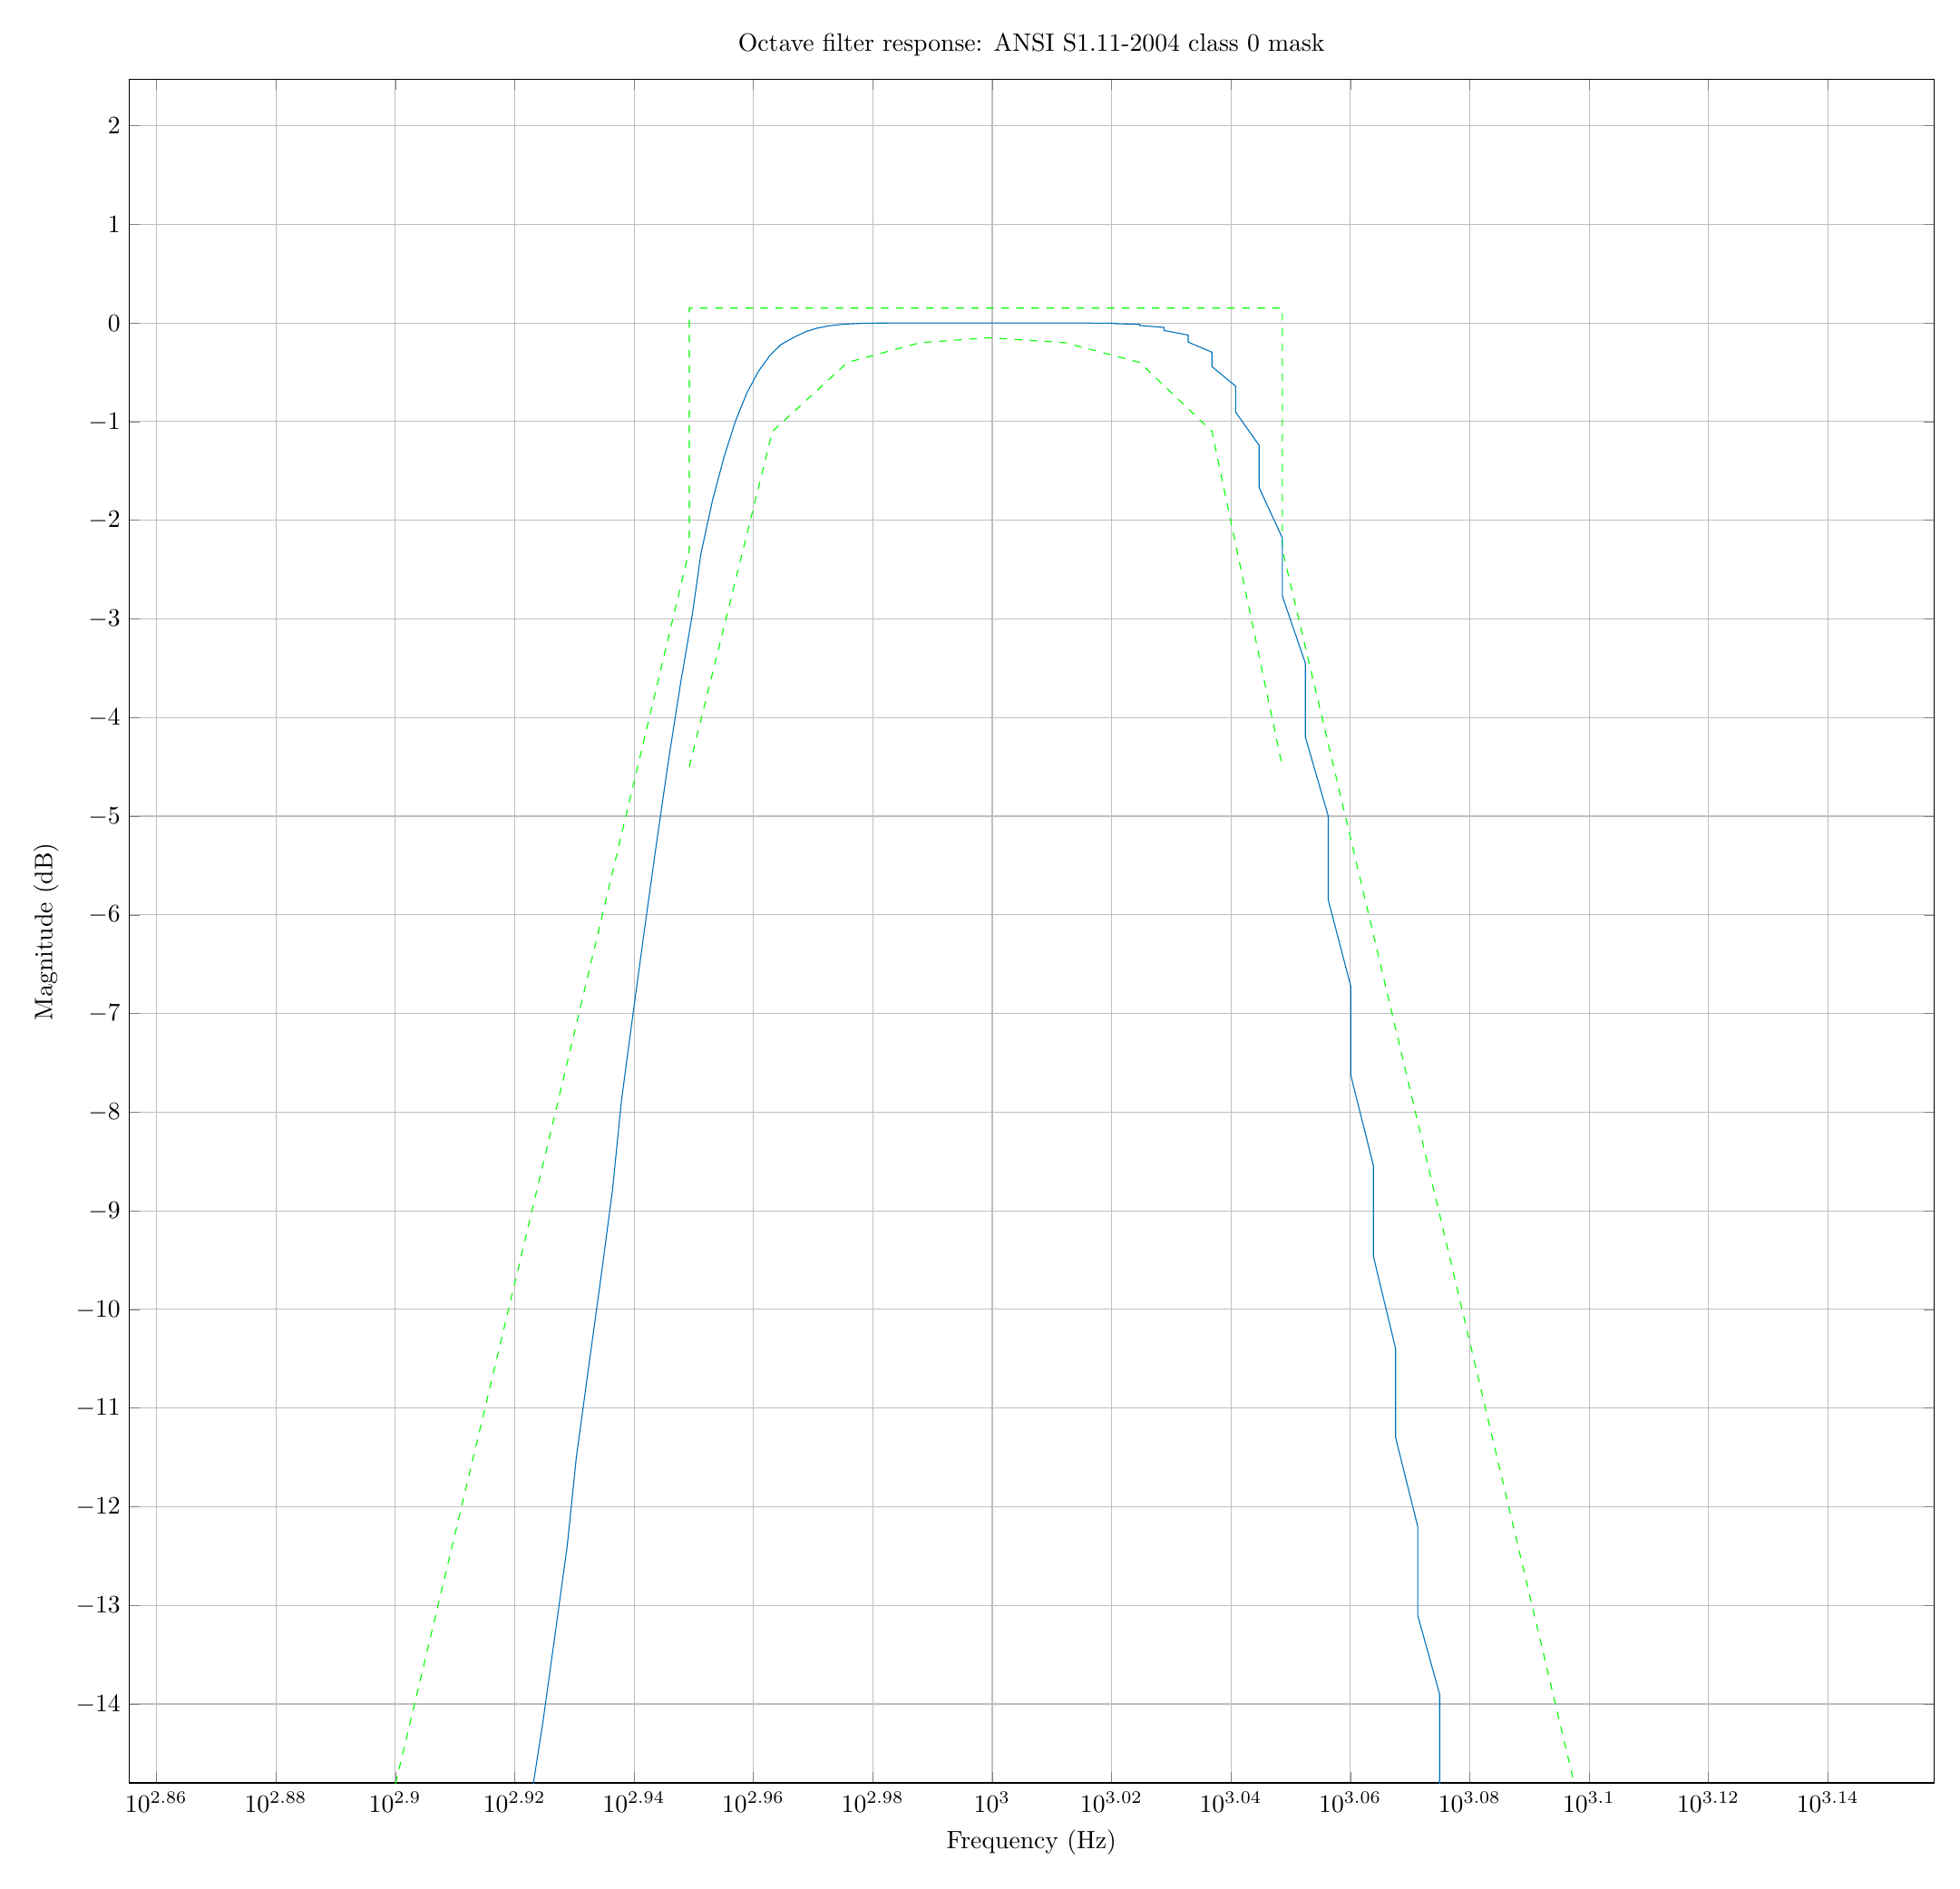
\begin{tikzpicture}

\begin{axis}[%
width=9.947in,
height=9.393in,
at={(0.448in,0.409in)},
scale only axis,
unbounded coords=jump,
xmode=log,
xmin=718,
xmax=1.44e+03,
xminorticks=true,
xlabel={Frequency (Hz)},
xmajorgrids,
xminorgrids,
ymin=-14.8,
ymax=2.47,
ylabel={Magnitude (dB)},
ymajorgrids,
axis background/.style={fill=white},
title={Octave filter response: ANSI S1.11-2004 class 0 mask}
]
\addplot [color=green,dashed,forget plot]
  table[row sep=crcr]{%
185	-75\\
327	-62\\
531	-42.5\\
773	-18\\
891	-2.3\\
891	0.15\\
920	0.15\\
947	0.15\\
974	0.15\\
1e+03	0.15\\
1.03e+03	0.15\\
1.06e+03	0.15\\
1.09e+03	0.15\\
1.12e+03	0.15\\
1.12e+03	-2.3\\
1.29e+03	-18\\
1.88e+03	-42.5\\
3.05e+03	-62\\
5.39e+03	-75\\
};
\addplot [color=green,dashed,forget plot]
  table[row sep=crcr]{%
185	nan\\
327	nan\\
531	nan\\
773	nan\\
891	-4.5\\
891	-4.5\\
920	-1.1\\
947	-0.4\\
974	-0.2\\
1e+03	-0.15\\
1.03e+03	-0.2\\
1.06e+03	-0.4\\
1.09e+03	-1.1\\
1.12e+03	-4.5\\
1.12e+03	-4.5\\
1.29e+03	nan\\
1.88e+03	nan\\
3.05e+03	nan\\
5.39e+03	nan\\
};
\addplot [color=mycolor1,solid,forget plot]
  table[row sep=crcr]{%
3	-253\\
3.01	-253\\
3.03	-252\\
3.04	-252\\
3.05	-252\\
3.07	-252\\
3.08	-252\\
3.09	-252\\
3.11	-252\\
3.12	-251\\
3.13	-251\\
3.15	-251\\
3.16	-251\\
3.18	-251\\
3.19	-251\\
3.2	-250\\
3.22	-250\\
3.23	-250\\
3.25	-250\\
3.26	-250\\
3.28	-250\\
3.29	-250\\
3.3	-249\\
3.32	-249\\
3.33	-249\\
3.35	-249\\
3.36	-249\\
3.38	-249\\
3.39	-248\\
3.41	-248\\
3.42	-248\\
3.44	-248\\
3.45	-248\\
3.47	-248\\
3.48	-248\\
3.5	-247\\
3.51	-247\\
3.53	-247\\
3.54	-247\\
3.56	-247\\
3.58	-247\\
3.59	-246\\
3.61	-246\\
3.62	-246\\
3.64	-246\\
3.66	-246\\
3.67	-246\\
3.69	-246\\
3.7	-245\\
3.72	-245\\
3.74	-245\\
3.75	-245\\
3.77	-245\\
3.79	-245\\
3.8	-244\\
3.82	-244\\
3.84	-244\\
3.85	-244\\
3.87	-244\\
3.89	-244\\
3.9	-244\\
3.92	-243\\
3.94	-243\\
3.96	-243\\
3.97	-243\\
3.99	-243\\
4.01	-243\\
4.03	-243\\
4.04	-242\\
4.06	-242\\
4.08	-242\\
4.1	-242\\
4.12	-242\\
4.13	-242\\
4.15	-241\\
4.17	-241\\
4.19	-241\\
4.21	-241\\
4.23	-241\\
4.24	-241\\
4.26	-241\\
4.28	-240\\
4.3	-240\\
4.32	-240\\
4.34	-240\\
4.36	-240\\
4.38	-240\\
4.4	-239\\
4.41	-239\\
4.43	-239\\
4.45	-239\\
4.47	-239\\
4.49	-239\\
4.51	-239\\
4.53	-238\\
4.55	-238\\
4.57	-238\\
4.59	-238\\
4.61	-238\\
4.63	-238\\
4.65	-237\\
4.67	-237\\
4.69	-237\\
4.72	-237\\
4.74	-237\\
4.76	-237\\
4.78	-237\\
4.8	-236\\
4.82	-236\\
4.84	-236\\
4.86	-236\\
4.88	-236\\
4.91	-236\\
4.93	-235\\
4.95	-235\\
4.97	-235\\
4.99	-235\\
5.01	-235\\
5.04	-235\\
5.06	-235\\
5.08	-234\\
5.1	-234\\
5.13	-234\\
5.15	-234\\
5.17	-234\\
5.19	-234\\
5.22	-234\\
5.24	-233\\
5.26	-233\\
5.29	-233\\
5.31	-233\\
5.33	-233\\
5.36	-233\\
5.38	-232\\
5.4	-232\\
5.43	-232\\
5.45	-232\\
5.47	-232\\
5.5	-232\\
5.52	-232\\
5.55	-231\\
5.57	-231\\
5.6	-231\\
5.62	-231\\
5.65	-231\\
5.67	-231\\
5.7	-230\\
5.72	-230\\
5.75	-230\\
5.77	-230\\
5.8	-230\\
5.82	-230\\
5.85	-230\\
5.87	-229\\
5.9	-229\\
5.92	-229\\
5.95	-229\\
5.98	-229\\
6	-229\\
6.03	-228\\
6.06	-228\\
6.08	-228\\
6.11	-228\\
6.14	-228\\
6.16	-228\\
6.19	-228\\
6.22	-227\\
6.25	-227\\
6.27	-227\\
6.3	-227\\
6.33	-227\\
6.36	-227\\
6.38	-226\\
6.41	-226\\
6.44	-226\\
6.47	-226\\
6.5	-226\\
6.53	-226\\
6.55	-226\\
6.58	-225\\
6.61	-225\\
6.64	-225\\
6.67	-225\\
6.7	-225\\
6.73	-225\\
6.76	-225\\
6.79	-224\\
6.82	-224\\
6.85	-224\\
6.88	-224\\
6.91	-224\\
6.94	-224\\
6.97	-223\\
7	-223\\
7.03	-223\\
7.06	-223\\
7.09	-223\\
7.12	-223\\
7.16	-223\\
7.19	-222\\
7.22	-222\\
7.25	-222\\
7.28	-222\\
7.31	-222\\
7.35	-222\\
7.38	-221\\
7.41	-221\\
7.44	-221\\
7.48	-221\\
7.51	-221\\
7.54	-221\\
7.58	-221\\
7.61	-220\\
7.64	-220\\
7.68	-220\\
7.71	-220\\
7.74	-220\\
7.78	-220\\
7.81	-219\\
7.85	-219\\
7.88	-219\\
7.92	-219\\
7.95	-219\\
7.99	-219\\
8.02	-219\\
8.06	-218\\
8.09	-218\\
8.13	-218\\
8.16	-218\\
8.2	-218\\
8.24	-218\\
8.27	-217\\
8.31	-217\\
8.34	-217\\
8.38	-217\\
8.42	-217\\
8.45	-217\\
8.49	-217\\
8.53	-216\\
8.57	-216\\
8.6	-216\\
8.64	-216\\
8.68	-216\\
8.72	-216\\
8.76	-216\\
8.8	-215\\
8.83	-215\\
8.87	-215\\
8.91	-215\\
8.95	-215\\
8.99	-215\\
9.03	-214\\
9.07	-214\\
9.11	-214\\
9.15	-214\\
9.19	-214\\
9.23	-214\\
9.27	-214\\
9.31	-213\\
9.35	-213\\
9.39	-213\\
9.44	-213\\
9.48	-213\\
9.52	-213\\
9.56	-212\\
9.6	-212\\
9.65	-212\\
9.69	-212\\
9.73	-212\\
9.77	-212\\
9.82	-212\\
9.86	-211\\
9.9	-211\\
9.95	-211\\
9.99	-211\\
10	-211\\
10.1	-211\\
10.1	-210\\
10.2	-210\\
10.2	-210\\
10.3	-210\\
10.3	-210\\
10.3	-210\\
10.4	-210\\
10.4	-209\\
10.5	-209\\
10.5	-209\\
10.6	-209\\
10.6	-209\\
10.7	-209\\
10.7	-208\\
10.8	-208\\
10.8	-208\\
10.9	-208\\
10.9	-208\\
11	-208\\
11	-208\\
11.1	-207\\
11.1	-207\\
11.1	-207\\
11.2	-207\\
11.2	-207\\
11.3	-207\\
11.3	-207\\
11.4	-206\\
11.4	-206\\
11.5	-206\\
11.5	-206\\
11.6	-206\\
11.6	-206\\
11.7	-205\\
11.8	-205\\
11.8	-205\\
11.9	-205\\
11.9	-205\\
12	-205\\
12	-205\\
12.1	-204\\
12.1	-204\\
12.2	-204\\
12.2	-204\\
12.3	-204\\
12.3	-204\\
12.4	-203\\
12.4	-203\\
12.5	-203\\
12.6	-203\\
12.6	-203\\
12.7	-203\\
12.7	-203\\
12.8	-202\\
12.8	-202\\
12.9	-202\\
12.9	-202\\
13	-202\\
13.1	-202\\
13.1	-201\\
13.2	-201\\
13.2	-201\\
13.3	-201\\
13.3	-201\\
13.4	-201\\
13.5	-201\\
13.5	-200\\
13.6	-200\\
13.6	-200\\
13.7	-200\\
13.8	-200\\
13.8	-200\\
13.9	-199\\
13.9	-199\\
14	-199\\
14.1	-199\\
14.1	-199\\
14.2	-199\\
14.3	-199\\
14.3	-198\\
14.4	-198\\
14.4	-198\\
14.5	-198\\
14.6	-198\\
14.6	-198\\
14.7	-198\\
14.8	-197\\
14.8	-197\\
14.9	-197\\
15	-197\\
15	-197\\
15.1	-197\\
15.2	-196\\
15.2	-196\\
15.3	-196\\
15.4	-196\\
15.4	-196\\
15.5	-196\\
15.6	-196\\
15.6	-195\\
15.7	-195\\
15.8	-195\\
15.8	-195\\
15.9	-195\\
16	-195\\
16.1	-194\\
16.1	-194\\
16.2	-194\\
16.3	-194\\
16.3	-194\\
16.4	-194\\
16.5	-194\\
16.6	-193\\
16.6	-193\\
16.7	-193\\
16.8	-193\\
16.8	-193\\
16.9	-193\\
17	-192\\
17.1	-192\\
17.1	-192\\
17.2	-192\\
17.3	-192\\
17.4	-192\\
17.4	-192\\
17.5	-191\\
17.6	-191\\
17.7	-191\\
17.8	-191\\
17.8	-191\\
17.9	-191\\
18	-190\\
18.1	-190\\
18.2	-190\\
18.2	-190\\
18.3	-190\\
18.4	-190\\
18.5	-190\\
18.6	-189\\
18.6	-189\\
18.7	-189\\
18.8	-189\\
18.9	-189\\
19	-189\\
19	-188\\
19.1	-188\\
19.2	-188\\
19.3	-188\\
19.4	-188\\
19.5	-188\\
19.6	-188\\
19.6	-187\\
19.7	-187\\
19.8	-187\\
19.9	-187\\
20	-187\\
20.1	-187\\
20.2	-187\\
20.3	-186\\
20.3	-186\\
20.4	-186\\
20.5	-186\\
20.6	-186\\
20.7	-186\\
20.8	-185\\
20.9	-185\\
21	-185\\
21.1	-185\\
21.2	-185\\
21.3	-185\\
21.4	-185\\
21.4	-184\\
21.5	-184\\
21.6	-184\\
21.7	-184\\
21.8	-184\\
21.9	-184\\
22	-183\\
22.1	-183\\
22.2	-183\\
22.3	-183\\
22.4	-183\\
22.5	-183\\
22.6	-183\\
22.7	-182\\
22.8	-182\\
22.9	-182\\
23	-182\\
23.1	-182\\
23.2	-182\\
23.3	-181\\
23.4	-181\\
23.5	-181\\
23.6	-181\\
23.7	-181\\
23.8	-181\\
23.9	-181\\
24	-180\\
24.1	-180\\
24.3	-180\\
24.4	-180\\
24.5	-180\\
24.6	-180\\
24.7	-179\\
24.8	-179\\
24.9	-179\\
25	-179\\
25.1	-179\\
25.2	-179\\
25.3	-179\\
25.5	-178\\
25.6	-178\\
25.7	-178\\
25.8	-178\\
25.9	-178\\
26	-178\\
26.1	-178\\
26.2	-177\\
26.4	-177\\
26.5	-177\\
26.6	-177\\
26.7	-177\\
26.8	-177\\
26.9	-176\\
27.1	-176\\
27.2	-176\\
27.3	-176\\
27.4	-176\\
27.5	-176\\
27.7	-176\\
27.8	-175\\
27.9	-175\\
28	-175\\
28.2	-175\\
28.3	-175\\
28.4	-175\\
28.5	-174\\
28.7	-174\\
28.8	-174\\
28.9	-174\\
29	-174\\
29.2	-174\\
29.3	-174\\
29.4	-173\\
29.5	-173\\
29.7	-173\\
29.8	-173\\
29.9	-173\\
30.1	-173\\
30.2	-172\\
30.3	-172\\
30.5	-172\\
30.6	-172\\
30.7	-172\\
30.9	-172\\
31	-172\\
31.1	-171\\
31.3	-171\\
31.4	-171\\
31.6	-171\\
31.7	-171\\
31.8	-171\\
32	-170\\
32.1	-170\\
32.3	-170\\
32.4	-170\\
32.5	-170\\
32.7	-170\\
32.8	-170\\
33	-169\\
33.1	-169\\
33.3	-169\\
33.4	-169\\
33.6	-169\\
33.7	-169\\
33.9	-168\\
34	-168\\
34.2	-168\\
34.3	-168\\
34.5	-168\\
34.6	-168\\
34.8	-168\\
34.9	-167\\
35.1	-167\\
35.2	-167\\
35.4	-167\\
35.5	-167\\
35.7	-167\\
35.8	-166\\
36	-166\\
36.2	-166\\
36.3	-166\\
36.5	-166\\
36.6	-166\\
36.8	-166\\
37	-165\\
37.1	-165\\
37.3	-165\\
37.5	-165\\
37.6	-165\\
37.8	-165\\
38	-165\\
38.1	-164\\
38.3	-164\\
38.5	-164\\
38.6	-164\\
38.8	-164\\
39	-164\\
39.1	-163\\
39.3	-163\\
39.5	-163\\
39.7	-163\\
39.8	-163\\
40	-163\\
40.2	-163\\
40.4	-162\\
40.5	-162\\
40.7	-162\\
40.9	-162\\
41.1	-162\\
41.3	-162\\
41.4	-161\\
41.6	-161\\
41.8	-161\\
42	-161\\
42.2	-161\\
42.4	-161\\
42.5	-161\\
42.7	-160\\
42.9	-160\\
43.1	-160\\
43.3	-160\\
43.5	-160\\
43.7	-160\\
43.9	-159\\
44.1	-159\\
44.3	-159\\
44.4	-159\\
44.6	-159\\
44.8	-159\\
45	-159\\
45.2	-158\\
45.4	-158\\
45.6	-158\\
45.8	-158\\
46	-158\\
46.2	-158\\
46.4	-157\\
46.6	-157\\
46.9	-157\\
47.1	-157\\
47.3	-157\\
47.5	-157\\
47.7	-157\\
47.9	-156\\
48.1	-156\\
48.3	-156\\
48.5	-156\\
48.7	-156\\
49	-156\\
49.2	-155\\
49.4	-155\\
49.6	-155\\
49.8	-155\\
50	-155\\
50.3	-155\\
50.5	-155\\
50.7	-154\\
50.9	-154\\
51.2	-154\\
51.4	-154\\
51.6	-154\\
51.8	-154\\
52.1	-153\\
52.3	-153\\
52.5	-153\\
52.7	-153\\
53	-153\\
53.2	-153\\
53.4	-153\\
53.7	-152\\
53.9	-152\\
54.2	-152\\
54.4	-152\\
54.6	-152\\
54.9	-152\\
55.1	-151\\
55.4	-151\\
55.6	-151\\
55.8	-151\\
56.1	-151\\
56.3	-151\\
56.6	-151\\
56.8	-150\\
57.1	-150\\
57.3	-150\\
57.6	-150\\
57.8	-150\\
58.1	-150\\
58.4	-149\\
58.6	-149\\
58.9	-149\\
59.1	-149\\
59.4	-149\\
59.6	-149\\
59.9	-149\\
60.2	-148\\
60.4	-148\\
60.7	-148\\
61	-148\\
61.2	-148\\
61.5	-148\\
61.8	-147\\
62.1	-147\\
62.3	-147\\
62.6	-147\\
62.9	-147\\
63.2	-147\\
63.4	-147\\
63.7	-146\\
64	-146\\
64.3	-146\\
64.6	-146\\
64.8	-146\\
65.1	-146\\
65.4	-145\\
65.7	-145\\
66	-145\\
66.3	-145\\
66.6	-145\\
66.9	-145\\
67.2	-145\\
67.5	-144\\
67.7	-144\\
68	-144\\
68.3	-144\\
68.6	-144\\
68.9	-144\\
69.3	-143\\
69.6	-143\\
69.9	-143\\
70.2	-143\\
70.5	-143\\
70.8	-143\\
71.1	-143\\
71.4	-142\\
71.7	-142\\
72	-142\\
72.4	-142\\
72.7	-142\\
73	-142\\
73.3	-141\\
73.6	-141\\
74	-141\\
74.3	-141\\
74.6	-141\\
74.9	-141\\
75.3	-141\\
75.6	-140\\
75.9	-140\\
76.3	-140\\
76.6	-140\\
76.9	-140\\
77.3	-140\\
77.6	-139\\
78	-139\\
78.3	-139\\
78.7	-139\\
79	-139\\
79.3	-139\\
79.7	-139\\
80	-138\\
80.4	-138\\
80.8	-138\\
81.1	-138\\
81.5	-138\\
81.8	-138\\
82.2	-137\\
82.5	-137\\
82.9	-137\\
83.3	-137\\
83.6	-137\\
84	-137\\
84.4	-137\\
84.8	-136\\
85.1	-136\\
85.5	-136\\
85.9	-136\\
86.3	-136\\
86.6	-136\\
87	-135\\
87.4	-135\\
87.8	-135\\
88.2	-135\\
88.6	-135\\
88.9	-135\\
89.3	-135\\
89.7	-134\\
90.1	-134\\
90.5	-134\\
90.9	-134\\
91.3	-134\\
91.7	-134\\
92.1	-133\\
92.5	-133\\
92.9	-133\\
93.3	-133\\
93.8	-133\\
94.2	-133\\
94.6	-133\\
95	-132\\
95.4	-132\\
95.8	-132\\
96.3	-132\\
96.7	-132\\
97.1	-132\\
97.5	-131\\
98	-131\\
98.4	-131\\
98.8	-131\\
99.3	-131\\
99.7	-131\\
100	-130\\
101	-130\\
101	-130\\
101	-130\\
102	-130\\
102	-130\\
103	-130\\
103	-129\\
104	-129\\
104	-129\\
105	-129\\
105	-129\\
106	-129\\
106	-128\\
106	-128\\
107	-128\\
107	-128\\
108	-128\\
108	-128\\
109	-128\\
109	-127\\
110	-127\\
110	-127\\
111	-127\\
111	-127\\
112	-127\\
112	-126\\
113	-126\\
113	-126\\
114	-126\\
114	-126\\
115	-126\\
115	-126\\
116	-125\\
116	-125\\
117	-125\\
117	-125\\
118	-125\\
118	-125\\
119	-124\\
119	-124\\
120	-124\\
120	-124\\
121	-124\\
121	-124\\
122	-123\\
123	-123\\
123	-123\\
124	-123\\
124	-123\\
125	-123\\
125	-123\\
126	-122\\
126	-122\\
127	-122\\
127	-122\\
128	-122\\
129	-122\\
129	-121\\
130	-121\\
130	-121\\
131	-121\\
131	-121\\
132	-121\\
133	-120\\
133	-120\\
134	-120\\
134	-120\\
135	-120\\
136	-120\\
136	-120\\
137	-119\\
137	-119\\
138	-119\\
139	-119\\
139	-119\\
140	-119\\
140	-118\\
141	-118\\
142	-118\\
142	-118\\
143	-118\\
144	-118\\
144	-117\\
145	-117\\
145	-117\\
146	-117\\
147	-117\\
147	-117\\
148	-117\\
149	-116\\
149	-116\\
150	-116\\
151	-116\\
151	-116\\
152	-116\\
153	-115\\
153	-115\\
154	-115\\
155	-115\\
155	-115\\
156	-115\\
157	-114\\
157	-114\\
158	-114\\
159	-114\\
159	-114\\
160	-114\\
161	-113\\
162	-113\\
162	-113\\
163	-113\\
164	-113\\
164	-113\\
165	-112\\
166	-112\\
167	-112\\
167	-112\\
168	-112\\
169	-112\\
170	-112\\
170	-111\\
171	-111\\
172	-111\\
173	-111\\
173	-111\\
174	-111\\
175	-110\\
176	-110\\
176	-110\\
177	-110\\
178	-110\\
179	-110\\
180	-109\\
180	-109\\
181	-109\\
182	-109\\
183	-109\\
184	-109\\
184	-108\\
185	-108\\
186	-108\\
187	-108\\
188	-108\\
188	-108\\
189	-107\\
190	-107\\
191	-107\\
192	-107\\
193	-107\\
193	-107\\
194	-106\\
195	-106\\
196	-106\\
197	-106\\
198	-106\\
199	-106\\
200	-105\\
200	-105\\
201	-105\\
202	-105\\
203	-105\\
204	-105\\
205	-104\\
206	-104\\
207	-104\\
208	-104\\
208	-104\\
209	-104\\
210	-103\\
211	-103\\
212	-103\\
213	-103\\
214	-103\\
215	-103\\
216	-102\\
217	-102\\
218	-102\\
219	-102\\
220	-102\\
221	-102\\
222	-101\\
223	-101\\
224	-101\\
225	-101\\
226	-101\\
227	-101\\
228	-100\\
229	-100\\
230	-100\\
231	-100\\
232	-99.8\\
233	-99.6\\
234	-99.5\\
235	-99.3\\
236	-99.1\\
237	-98.9\\
238	-98.8\\
239	-98.6\\
240	-98.4\\
241	-98.3\\
242	-98.1\\
243	-97.9\\
244	-97.8\\
245	-97.6\\
246	-97.4\\
247	-97.2\\
248	-97.1\\
250	-96.9\\
251	-96.7\\
252	-96.5\\
253	-96.4\\
254	-96.2\\
255	-96\\
256	-95.8\\
257	-95.7\\
258	-95.5\\
260	-95.3\\
261	-95.2\\
262	-95\\
263	-94.8\\
264	-94.6\\
265	-94.5\\
267	-94.3\\
268	-94.1\\
269	-93.9\\
270	-93.7\\
271	-93.6\\
272	-93.4\\
274	-93.2\\
275	-93\\
276	-92.9\\
277	-92.7\\
279	-92.5\\
280	-92.3\\
281	-92.1\\
282	-92\\
283	-91.8\\
285	-91.6\\
286	-91.4\\
287	-91.3\\
288	-91.1\\
290	-90.9\\
291	-90.7\\
292	-90.5\\
294	-90.3\\
295	-90.2\\
296	-90\\
297	-89.8\\
299	-89.6\\
300	-89.4\\
301	-89.3\\
303	-89.1\\
304	-88.9\\
305	-88.7\\
307	-88.5\\
308	-88.3\\
309	-88.2\\
311	-88\\
312	-87.8\\
314	-87.6\\
315	-87.4\\
316	-87.2\\
318	-87\\
319	-86.9\\
321	-86.7\\
322	-86.5\\
323	-86.3\\
325	-86.1\\
326	-85.9\\
328	-85.7\\
329	-85.5\\
331	-85.3\\
332	-85.2\\
333	-85\\
335	-84.8\\
336	-84.6\\
338	-84.4\\
339	-84.2\\
341	-84\\
342	-83.8\\
344	-83.6\\
345	-83.4\\
347	-83.2\\
348	-83\\
350	-82.8\\
352	-82.6\\
353	-82.5\\
355	-82.3\\
356	-82.1\\
358	-81.9\\
359	-81.7\\
361	-81.5\\
362	-81.3\\
364	-81.1\\
366	-80.9\\
367	-80.7\\
369	-80.5\\
371	-80.3\\
372	-80.1\\
374	-79.9\\
375	-79.7\\
377	-79.5\\
379	-79.3\\
380	-79.1\\
382	-78.8\\
384	-78.6\\
385	-78.4\\
387	-78.2\\
389	-78\\
391	-77.8\\
392	-77.6\\
394	-77.4\\
396	-77.2\\
397	-77\\
399	-76.8\\
401	-76.6\\
403	-76.4\\
405	-76.1\\
406	-75.9\\
408	-75.7\\
410	-75.5\\
412	-75.3\\
414	-75.1\\
415	-74.9\\
417	-74.6\\
419	-74.4\\
421	-74.2\\
423	-74\\
425	-73.8\\
426	-73.5\\
428	-73.3\\
430	-73.1\\
432	-72.9\\
434	-72.7\\
436	-72.4\\
438	-72.2\\
440	-72\\
442	-71.8\\
444	-71.5\\
446	-71.3\\
448	-71.1\\
449	-70.8\\
451	-70.6\\
453	-70.4\\
455	-70.2\\
457	-69.9\\
459	-69.7\\
461	-69.5\\
464	-69.2\\
466	-69\\
468	-68.7\\
470	-68.5\\
472	-68.3\\
474	-68\\
476	-67.8\\
478	-67.5\\
480	-67.3\\
482	-67.1\\
484	-66.8\\
486	-66.6\\
489	-66.3\\
491	-66.1\\
493	-65.8\\
495	-65.6\\
497	-65.3\\
499	-65.1\\
502	-64.8\\
504	-64.6\\
506	-64.3\\
508	-64\\
511	-63.8\\
513	-63.5\\
515	-63.3\\
517	-63\\
520	-62.7\\
522	-62.5\\
524	-62.2\\
526	-61.9\\
529	-61.7\\
531	-61.4\\
533	-61.1\\
536	-60.8\\
538	-60.6\\
540	-60.3\\
543	-60\\
545	-59.7\\
548	-59.4\\
550	-59.2\\
552	-58.9\\
555	-58.6\\
557	-58.3\\
560	-58\\
562	-57.7\\
565	-57.4\\
567	-57.1\\
570	-56.8\\
572	-56.5\\
575	-56.2\\
577	-55.9\\
580	-55.6\\
582	-55.3\\
585	-55\\
588	-54.7\\
590	-54.4\\
593	-54.1\\
595	-53.7\\
598	-53.4\\
601	-53.1\\
603	-52.8\\
606	-52.4\\
609	-52.1\\
611	-51.8\\
614	-51.4\\
617	-51.1\\
619	-50.8\\
622	-50.4\\
625	-50.1\\
628	-49.7\\
630	-49.4\\
633	-49\\
636	-48.7\\
639	-48.3\\
641	-47.9\\
644	-47.6\\
647	-47.2\\
650	-46.8\\
653	-46.4\\
656	-46.1\\
659	-45.7\\
661	-45.3\\
664	-44.9\\
667	-44.5\\
670	-44.1\\
673	-43.7\\
676	-43.3\\
679	-42.9\\
682	-42.5\\
685	-42\\
688	-41.6\\
691	-41.2\\
694	-40.8\\
697	-40.3\\
700	-39.9\\
703	-39.4\\
706	-39\\
710	-38.5\\
713	-38.1\\
716	-37.6\\
719	-37.1\\
722	-36.6\\
725	-36.1\\
729	-35.6\\
732	-35.1\\
735	-34.6\\
738	-34.1\\
741	-33.6\\
745	-33.1\\
748	-32.5\\
751	-32\\
755	-31.4\\
758	-30.9\\
761	-30.3\\
765	-29.7\\
768	-29.2\\
771	-28.6\\
775	-28\\
778	-27.3\\
782	-26.7\\
785	-26.1\\
788	-25.4\\
792	-24.8\\
795	-24.1\\
799	-23.4\\
802	-22.7\\
806	-22\\
809	-21.3\\
813	-20.6\\
817	-19.8\\
820	-19.1\\
824	-18.3\\
827	-17.5\\
831	-16.7\\
835	-15.9\\
838	-15\\
842	-14.2\\
846	-13.3\\
850	-12.4\\
853	-11.5\\
857	-10.6\\
861	-9.71\\
865	-8.79\\
868	-7.88\\
872	-6.97\\
876	-6.09\\
880	-5.23\\
884	-4.41\\
888	-3.65\\
892	-2.96\\
895	-2.34\\
899	-1.8\\
903	-1.36\\
907	-0.994\\
911	-0.709\\
915	-0.493\\
919	-0.334\\
923	-0.22\\
928	-0.141\\
932	-0.0878\\
936	-0.0528\\
940	-0.0306\\
944	-0.0171\\
948	-0.00906\\
952	-0.00456\\
956	-0.00215\\
961	-0.000937\\
965	-0.000371\\
969	-0.00013\\
973	-3.9e-05\\
978	-9.42e-06\\
982	-1.67e-06\\
986	-1.84e-07\\
991	-8.72e-09\\
995	1.77e-10\\
999	2.52e-10\\
1e+03	5.94e-11\\
1.01e+03	-2.5e-09\\
1.01e+03	-8.33e-08\\
1.02e+03	-9.25e-07\\
1.02e+03	-5.86e-06\\
1.03e+03	-2.63e-05\\
1.03e+03	-9.29e-05\\
1.04e+03	-0.000276\\
1.04e+03	-0.000721\\
1.04e+03	-0.0017\\
1.05e+03	-0.00368\\
1.05e+03	-0.00746\\
1.06e+03	-0.0143\\
1.06e+03	-0.0259\\
1.07e+03	-0.0453\\
1.07e+03	-0.076\\
1.08e+03	-0.123\\
1.08e+03	-0.194\\
1.09e+03	-0.297\\
1.09e+03	-0.443\\
1.1e+03	-0.641\\
1.1e+03	-0.905\\
1.11e+03	-1.24\\
1.11e+03	-1.67\\
1.12e+03	-2.18\\
1.12e+03	-2.77\\
1.13e+03	-3.45\\
1.13e+03	-4.2\\
1.14e+03	-5\\
1.14e+03	-5.85\\
1.15e+03	-6.73\\
1.15e+03	-7.63\\
1.16e+03	-8.54\\
1.16e+03	-9.46\\
1.17e+03	-10.4\\
1.17e+03	-11.3\\
1.18e+03	-12.2\\
1.18e+03	-13.1\\
1.19e+03	-13.9\\
1.19e+03	-14.8\\
1.2e+03	-15.7\\
1.2e+03	-16.5\\
1.21e+03	-17.3\\
1.21e+03	-18.1\\
1.22e+03	-18.9\\
1.22e+03	-19.6\\
1.23e+03	-20.4\\
1.23e+03	-21.1\\
1.24e+03	-21.9\\
1.24e+03	-22.6\\
1.25e+03	-23.3\\
1.26e+03	-24\\
1.26e+03	-24.6\\
1.27e+03	-25.3\\
1.27e+03	-25.9\\
1.28e+03	-26.6\\
1.28e+03	-27.2\\
1.29e+03	-27.8\\
1.29e+03	-28.4\\
1.3e+03	-29\\
1.31e+03	-29.6\\
1.31e+03	-30.2\\
1.32e+03	-30.8\\
1.32e+03	-31.3\\
1.33e+03	-31.9\\
1.34e+03	-32.4\\
1.34e+03	-33\\
1.35e+03	-33.5\\
1.35e+03	-34\\
1.36e+03	-34.5\\
1.36e+03	-35.1\\
1.37e+03	-35.6\\
1.38e+03	-36.1\\
1.38e+03	-36.5\\
1.39e+03	-37\\
1.4e+03	-37.5\\
1.4e+03	-38\\
1.41e+03	-38.5\\
1.41e+03	-38.9\\
1.42e+03	-39.4\\
1.43e+03	-39.8\\
1.43e+03	-40.3\\
1.44e+03	-40.7\\
1.45e+03	-41.1\\
1.45e+03	-41.6\\
1.46e+03	-42\\
1.46e+03	-42.4\\
1.47e+03	-42.8\\
1.48e+03	-43.3\\
1.48e+03	-43.7\\
1.49e+03	-44.1\\
1.5e+03	-44.5\\
1.5e+03	-44.9\\
1.51e+03	-45.3\\
1.52e+03	-45.7\\
1.52e+03	-46\\
1.53e+03	-46.4\\
1.54e+03	-46.8\\
1.54e+03	-47.2\\
1.55e+03	-47.6\\
1.56e+03	-47.9\\
1.56e+03	-48.3\\
1.57e+03	-48.7\\
1.58e+03	-49\\
1.58e+03	-49.4\\
1.59e+03	-49.7\\
1.6e+03	-50.1\\
1.61e+03	-50.4\\
1.61e+03	-50.8\\
1.62e+03	-51.1\\
1.63e+03	-51.4\\
1.63e+03	-51.8\\
1.64e+03	-52.1\\
1.65e+03	-52.5\\
1.66e+03	-52.8\\
1.66e+03	-53.1\\
1.67e+03	-53.4\\
1.68e+03	-53.8\\
1.69e+03	-54.1\\
1.69e+03	-54.4\\
1.7e+03	-54.7\\
1.71e+03	-55\\
1.71e+03	-55.3\\
1.72e+03	-55.7\\
1.73e+03	-56\\
1.74e+03	-56.3\\
1.75e+03	-56.6\\
1.75e+03	-56.9\\
1.76e+03	-57.2\\
1.77e+03	-57.5\\
1.78e+03	-57.8\\
1.78e+03	-58.1\\
1.79e+03	-58.4\\
1.8e+03	-58.6\\
1.81e+03	-58.9\\
1.82e+03	-59.2\\
1.82e+03	-59.5\\
1.83e+03	-59.8\\
1.84e+03	-60.1\\
1.85e+03	-60.4\\
1.86e+03	-60.6\\
1.86e+03	-60.9\\
1.87e+03	-61.2\\
1.88e+03	-61.5\\
1.89e+03	-61.7\\
1.9e+03	-62\\
1.91e+03	-62.3\\
1.91e+03	-62.6\\
1.92e+03	-62.8\\
1.93e+03	-63.1\\
1.94e+03	-63.4\\
1.95e+03	-63.6\\
1.96e+03	-63.9\\
1.97e+03	-64.1\\
1.97e+03	-64.4\\
1.98e+03	-64.7\\
1.99e+03	-64.9\\
2e+03	-65.2\\
2.01e+03	-65.4\\
2.02e+03	-65.7\\
2.03e+03	-65.9\\
2.04e+03	-66.2\\
2.04e+03	-66.4\\
2.05e+03	-66.7\\
2.06e+03	-66.9\\
2.07e+03	-67.2\\
2.08e+03	-67.4\\
2.09e+03	-67.7\\
2.1e+03	-67.9\\
2.11e+03	-68.2\\
2.12e+03	-68.4\\
2.13e+03	-68.7\\
2.14e+03	-68.9\\
2.15e+03	-69.1\\
2.15e+03	-69.4\\
2.16e+03	-69.6\\
2.17e+03	-69.8\\
2.18e+03	-70.1\\
2.19e+03	-70.3\\
2.2e+03	-70.6\\
2.21e+03	-70.8\\
2.22e+03	-71\\
2.23e+03	-71.2\\
2.24e+03	-71.5\\
2.25e+03	-71.7\\
2.26e+03	-71.9\\
2.27e+03	-72.2\\
2.28e+03	-72.4\\
2.29e+03	-72.6\\
2.3e+03	-72.8\\
2.31e+03	-73.1\\
2.32e+03	-73.3\\
2.33e+03	-73.5\\
2.34e+03	-73.7\\
2.35e+03	-74\\
2.36e+03	-74.2\\
2.37e+03	-74.4\\
2.38e+03	-74.6\\
2.39e+03	-74.9\\
2.4e+03	-75.1\\
2.42e+03	-75.3\\
2.43e+03	-75.5\\
2.44e+03	-75.7\\
2.45e+03	-75.9\\
2.46e+03	-76.2\\
2.47e+03	-76.4\\
2.48e+03	-76.6\\
2.49e+03	-76.8\\
2.5e+03	-77\\
2.51e+03	-77.2\\
2.52e+03	-77.4\\
2.53e+03	-77.7\\
2.55e+03	-77.9\\
2.56e+03	-78.1\\
2.57e+03	-78.3\\
2.58e+03	-78.5\\
2.59e+03	-78.7\\
2.6e+03	-78.9\\
2.61e+03	-79.1\\
2.63e+03	-79.3\\
2.64e+03	-79.5\\
2.65e+03	-79.7\\
2.66e+03	-79.9\\
2.67e+03	-80.2\\
2.68e+03	-80.4\\
2.7e+03	-80.6\\
2.71e+03	-80.8\\
2.72e+03	-81\\
2.73e+03	-81.2\\
2.74e+03	-81.4\\
2.76e+03	-81.6\\
2.77e+03	-81.8\\
2.78e+03	-82\\
2.79e+03	-82.2\\
2.8e+03	-82.4\\
2.82e+03	-82.6\\
2.83e+03	-82.8\\
2.84e+03	-83\\
2.85e+03	-83.2\\
2.87e+03	-83.4\\
2.88e+03	-83.6\\
2.89e+03	-83.8\\
2.9e+03	-84\\
2.92e+03	-84.2\\
2.93e+03	-84.4\\
2.94e+03	-84.6\\
2.96e+03	-84.8\\
2.97e+03	-85\\
2.98e+03	-85.2\\
3e+03	-85.3\\
3.01e+03	-85.5\\
3.02e+03	-85.7\\
3.03e+03	-85.9\\
3.05e+03	-86.1\\
3.06e+03	-86.3\\
3.08e+03	-86.5\\
3.09e+03	-86.7\\
3.1e+03	-86.9\\
3.12e+03	-87.1\\
3.13e+03	-87.3\\
3.14e+03	-87.5\\
3.16e+03	-87.7\\
3.17e+03	-87.9\\
3.19e+03	-88\\
3.2e+03	-88.2\\
3.21e+03	-88.4\\
3.23e+03	-88.6\\
3.24e+03	-88.8\\
3.26e+03	-89\\
3.27e+03	-89.2\\
3.28e+03	-89.4\\
3.3e+03	-89.6\\
3.31e+03	-89.7\\
3.33e+03	-89.9\\
3.34e+03	-90.1\\
3.36e+03	-90.3\\
3.37e+03	-90.5\\
3.39e+03	-90.7\\
3.4e+03	-90.9\\
3.42e+03	-91.1\\
3.43e+03	-91.2\\
3.45e+03	-91.4\\
3.46e+03	-91.6\\
3.48e+03	-91.8\\
3.49e+03	-92\\
3.51e+03	-92.2\\
3.52e+03	-92.4\\
3.54e+03	-92.5\\
3.55e+03	-92.7\\
3.57e+03	-92.9\\
3.59e+03	-93.1\\
3.6e+03	-93.3\\
3.62e+03	-93.5\\
3.63e+03	-93.6\\
3.65e+03	-93.8\\
3.67e+03	-94\\
3.68e+03	-94.2\\
3.7e+03	-94.4\\
3.71e+03	-94.6\\
3.73e+03	-94.7\\
3.75e+03	-94.9\\
3.76e+03	-95.1\\
3.78e+03	-95.3\\
3.8e+03	-95.5\\
3.81e+03	-95.7\\
3.83e+03	-95.8\\
3.85e+03	-96\\
3.86e+03	-96.2\\
3.88e+03	-96.4\\
3.9e+03	-96.6\\
3.91e+03	-96.7\\
3.93e+03	-96.9\\
3.95e+03	-97.1\\
3.97e+03	-97.3\\
3.98e+03	-97.5\\
4e+03	-97.6\\
4.02e+03	-97.8\\
4.04e+03	-98\\
4.05e+03	-98.2\\
4.07e+03	-98.4\\
4.09e+03	-98.5\\
4.11e+03	-98.7\\
4.13e+03	-98.9\\
4.14e+03	-99.1\\
4.16e+03	-99.3\\
4.18e+03	-99.4\\
4.2e+03	-99.6\\
4.22e+03	-99.8\\
4.24e+03	-100\\
4.26e+03	-100\\
4.27e+03	-100\\
4.29e+03	-101\\
4.31e+03	-101\\
4.33e+03	-101\\
4.35e+03	-101\\
4.37e+03	-101\\
4.39e+03	-101\\
4.41e+03	-102\\
4.43e+03	-102\\
4.45e+03	-102\\
4.47e+03	-102\\
4.49e+03	-102\\
4.51e+03	-102\\
4.53e+03	-103\\
4.55e+03	-103\\
4.57e+03	-103\\
4.59e+03	-103\\
4.61e+03	-103\\
4.63e+03	-104\\
4.65e+03	-104\\
4.67e+03	-104\\
4.69e+03	-104\\
4.71e+03	-104\\
4.73e+03	-104\\
4.75e+03	-105\\
4.77e+03	-105\\
4.79e+03	-105\\
4.81e+03	-105\\
4.83e+03	-105\\
4.85e+03	-105\\
4.88e+03	-106\\
4.9e+03	-106\\
4.92e+03	-106\\
4.94e+03	-106\\
4.96e+03	-106\\
4.98e+03	-107\\
5.01e+03	-107\\
5.03e+03	-107\\
5.05e+03	-107\\
5.07e+03	-107\\
5.09e+03	-107\\
5.12e+03	-108\\
5.14e+03	-108\\
5.16e+03	-108\\
5.19e+03	-108\\
5.21e+03	-108\\
5.23e+03	-108\\
5.25e+03	-109\\
5.28e+03	-109\\
5.3e+03	-109\\
5.32e+03	-109\\
5.35e+03	-109\\
5.37e+03	-110\\
5.39e+03	-110\\
5.42e+03	-110\\
5.44e+03	-110\\
5.47e+03	-110\\
5.49e+03	-110\\
5.51e+03	-111\\
5.54e+03	-111\\
5.56e+03	-111\\
5.59e+03	-111\\
5.61e+03	-111\\
5.64e+03	-111\\
5.66e+03	-112\\
5.69e+03	-112\\
5.71e+03	-112\\
5.74e+03	-112\\
5.76e+03	-112\\
5.79e+03	-113\\
5.81e+03	-113\\
5.84e+03	-113\\
5.86e+03	-113\\
5.89e+03	-113\\
5.92e+03	-113\\
5.94e+03	-114\\
5.97e+03	-114\\
5.99e+03	-114\\
6.02e+03	-114\\
6.05e+03	-114\\
6.07e+03	-115\\
6.1e+03	-115\\
6.13e+03	-115\\
6.15e+03	-115\\
6.18e+03	-115\\
6.21e+03	-115\\
6.24e+03	-116\\
6.26e+03	-116\\
6.29e+03	-116\\
6.32e+03	-116\\
6.35e+03	-116\\
6.37e+03	-116\\
6.4e+03	-117\\
6.43e+03	-117\\
6.46e+03	-117\\
6.49e+03	-117\\
6.51e+03	-117\\
6.54e+03	-118\\
6.57e+03	-118\\
6.6e+03	-118\\
6.63e+03	-118\\
6.66e+03	-118\\
6.69e+03	-118\\
6.72e+03	-119\\
6.75e+03	-119\\
6.78e+03	-119\\
6.81e+03	-119\\
6.84e+03	-119\\
6.87e+03	-120\\
6.9e+03	-120\\
6.93e+03	-120\\
6.96e+03	-120\\
6.99e+03	-120\\
7.02e+03	-120\\
7.05e+03	-121\\
7.08e+03	-121\\
7.11e+03	-121\\
7.14e+03	-121\\
7.18e+03	-121\\
7.21e+03	-122\\
7.24e+03	-122\\
7.27e+03	-122\\
7.3e+03	-122\\
7.33e+03	-122\\
7.37e+03	-122\\
7.4e+03	-123\\
7.43e+03	-123\\
7.46e+03	-123\\
7.5e+03	-123\\
7.53e+03	-123\\
7.56e+03	-124\\
7.6e+03	-124\\
7.63e+03	-124\\
7.66e+03	-124\\
7.7e+03	-124\\
7.73e+03	-125\\
7.77e+03	-125\\
7.8e+03	-125\\
7.83e+03	-125\\
7.87e+03	-125\\
7.9e+03	-125\\
7.94e+03	-126\\
7.97e+03	-126\\
8.01e+03	-126\\
8.04e+03	-126\\
8.08e+03	-126\\
8.11e+03	-127\\
8.15e+03	-127\\
8.19e+03	-127\\
8.22e+03	-127\\
8.26e+03	-127\\
8.29e+03	-128\\
8.33e+03	-128\\
8.37e+03	-128\\
8.4e+03	-128\\
8.44e+03	-128\\
8.48e+03	-129\\
8.52e+03	-129\\
8.55e+03	-129\\
8.59e+03	-129\\
8.63e+03	-129\\
8.67e+03	-129\\
8.7e+03	-130\\
8.74e+03	-130\\
8.78e+03	-130\\
8.82e+03	-130\\
8.86e+03	-130\\
8.9e+03	-131\\
8.94e+03	-131\\
8.98e+03	-131\\
9.02e+03	-131\\
9.06e+03	-131\\
9.1e+03	-132\\
9.14e+03	-132\\
9.18e+03	-132\\
9.22e+03	-132\\
9.26e+03	-132\\
9.3e+03	-133\\
9.34e+03	-133\\
9.38e+03	-133\\
9.42e+03	-133\\
9.46e+03	-133\\
9.5e+03	-134\\
9.55e+03	-134\\
9.59e+03	-134\\
9.63e+03	-134\\
9.67e+03	-134\\
9.71e+03	-135\\
9.76e+03	-135\\
9.8e+03	-135\\
9.84e+03	-135\\
9.89e+03	-136\\
9.93e+03	-136\\
9.97e+03	-136\\
1e+04	-136\\
1.01e+04	-136\\
1.01e+04	-137\\
1.02e+04	-137\\
1.02e+04	-137\\
1.02e+04	-137\\
1.03e+04	-137\\
1.03e+04	-138\\
1.04e+04	-138\\
1.04e+04	-138\\
1.05e+04	-138\\
1.05e+04	-138\\
1.06e+04	-139\\
1.06e+04	-139\\
1.07e+04	-139\\
1.07e+04	-139\\
1.07e+04	-140\\
1.08e+04	-140\\
1.08e+04	-140\\
1.09e+04	-140\\
1.09e+04	-140\\
1.1e+04	-141\\
1.1e+04	-141\\
1.11e+04	-141\\
1.11e+04	-141\\
1.12e+04	-142\\
1.12e+04	-142\\
1.13e+04	-142\\
1.13e+04	-142\\
1.14e+04	-143\\
1.14e+04	-143\\
1.15e+04	-143\\
1.15e+04	-143\\
1.16e+04	-143\\
1.16e+04	-144\\
1.17e+04	-144\\
1.17e+04	-144\\
1.18e+04	-144\\
1.18e+04	-145\\
1.19e+04	-145\\
1.19e+04	-145\\
1.2e+04	-145\\
1.2e+04	-146\\
1.21e+04	-146\\
1.22e+04	-146\\
1.22e+04	-146\\
1.23e+04	-147\\
1.23e+04	-147\\
1.24e+04	-147\\
1.24e+04	-147\\
1.25e+04	-148\\
1.25e+04	-148\\
1.26e+04	-148\\
1.26e+04	-148\\
1.27e+04	-149\\
1.28e+04	-149\\
1.28e+04	-149\\
1.29e+04	-149\\
1.29e+04	-150\\
1.3e+04	-150\\
1.3e+04	-150\\
1.31e+04	-150\\
1.32e+04	-151\\
1.32e+04	-151\\
1.33e+04	-151\\
1.33e+04	-151\\
1.34e+04	-152\\
1.34e+04	-152\\
1.35e+04	-152\\
1.36e+04	-153\\
1.36e+04	-153\\
1.37e+04	-153\\
1.37e+04	-153\\
1.38e+04	-154\\
1.39e+04	-154\\
1.39e+04	-154\\
1.4e+04	-155\\
1.4e+04	-155\\
1.41e+04	-155\\
1.42e+04	-155\\
1.42e+04	-156\\
1.43e+04	-156\\
1.44e+04	-156\\
1.44e+04	-157\\
1.45e+04	-157\\
1.45e+04	-157\\
1.46e+04	-158\\
1.47e+04	-158\\
1.47e+04	-158\\
1.48e+04	-159\\
1.49e+04	-159\\
1.49e+04	-159\\
1.5e+04	-159\\
1.51e+04	-160\\
1.51e+04	-160\\
1.52e+04	-160\\
1.53e+04	-161\\
1.53e+04	-161\\
1.54e+04	-161\\
1.55e+04	-162\\
1.55e+04	-162\\
1.56e+04	-163\\
1.57e+04	-163\\
1.57e+04	-163\\
1.58e+04	-164\\
1.59e+04	-164\\
1.6e+04	-164\\
1.6e+04	-165\\
1.61e+04	-165\\
1.62e+04	-165\\
1.62e+04	-166\\
1.63e+04	-166\\
1.64e+04	-167\\
1.65e+04	-167\\
1.65e+04	-167\\
1.66e+04	-168\\
1.67e+04	-168\\
1.67e+04	-169\\
1.68e+04	-169\\
1.69e+04	-169\\
1.7e+04	-170\\
1.7e+04	-170\\
1.71e+04	-171\\
1.72e+04	-171\\
1.73e+04	-172\\
1.73e+04	-172\\
1.74e+04	-173\\
1.75e+04	-173\\
1.76e+04	-173\\
1.76e+04	-174\\
1.77e+04	-174\\
1.78e+04	-175\\
1.79e+04	-175\\
1.8e+04	-176\\
1.8e+04	-176\\
1.81e+04	-177\\
1.82e+04	-177\\
1.83e+04	-178\\
1.84e+04	-179\\
1.84e+04	-179\\
1.85e+04	-180\\
1.86e+04	-180\\
1.87e+04	-181\\
1.88e+04	-181\\
1.89e+04	-182\\
1.89e+04	-183\\
1.9e+04	-183\\
1.91e+04	-184\\
1.92e+04	-184\\
1.93e+04	-185\\
1.94e+04	-186\\
1.94e+04	-186\\
1.95e+04	-187\\
1.96e+04	-188\\
1.97e+04	-189\\
1.98e+04	-189\\
1.99e+04	-190\\
2e+04	-191\\
2e+04	-192\\
2.01e+04	-193\\
2.02e+04	-193\\
2.03e+04	-194\\
2.04e+04	-195\\
2.05e+04	-196\\
2.06e+04	-197\\
2.07e+04	-198\\
2.08e+04	-199\\
2.09e+04	-200\\
2.09e+04	-201\\
2.1e+04	-202\\
2.11e+04	-203\\
2.12e+04	-204\\
2.13e+04	-206\\
2.14e+04	-207\\
2.15e+04	-208\\
2.16e+04	-210\\
2.17e+04	-211\\
2.18e+04	-212\\
2.19e+04	-214\\
2.2e+04	-216\\
2.21e+04	-217\\
2.22e+04	-219\\
2.23e+04	-221\\
2.24e+04	-223\\
2.25e+04	-225\\
2.26e+04	-228\\
2.27e+04	-230\\
2.28e+04	-233\\
2.29e+04	-236\\
2.3e+04	-239\\
2.31e+04	-243\\
2.32e+04	-247\\
2.33e+04	-251\\
2.34e+04	-257\\
2.35e+04	-263\\
2.36e+04	-271\\
2.37e+04	-280\\
2.38e+04	-294\\
2.39e+04	-319\\
2.4e+04	-inf\\
};
\end{axis}
\end{tikzpicture}%
	\caption{A filter-bank with center frequency in 1 $k$Hz displayed with class 0 mask requirements.}
	\label{fig:1000KhzFilterClass0}
\end{figure}

\subsection{Procedure}

The response of each ANC system is done by calculating the magnitude difference, when the system is turned on and off. This is done for all bands separately.  
\\
Listing \ref{lst:filterbanksProcedure} shows the procedure used to calculate each output of the filter. The filters takes the recorded signal as input and outputs the filtered response. An RMS value of each filter-bank is then calculated. Using the RMS value of each band, the ratio between on and off is then determined. 

\begin{lstlisting} [language=MATLAB, caption=Calculation of each filter with averaging and comparison. , label={lst:filterbanksProcedure}]
for i=1:Nfc
  ThirdoctFilt = FilterBank{i};  
  yBasisoff(:,i) = ThirdoctFilt(Basisoff);
  yBasisOn(:,i) = ThirdoctFilt(BasisOn); 
  yLPoff(:,i) = ThirdoctFilt(LPoff);
  yLPon(:,i) = ThirdoctFilt(LPon);    
end
% Average the output of the filter and compare
rmsBasisoff = rms(yBasisoff);
rmsBasisOn  = rms(yBasisOn);
Difference(1,:)=-20*log10(rmsBasisOn./rmsBasisoff);
  
rmsLPoff = rms(yLPoff);
rmsLPon  = rms(yLPon);
Difference(2,:)=-20*log10(rmsLPon./rmsLPoff);
\end{lstlisting}

%When the ratio is determined, 
%
%\ref{lst:filterbanksPlot}
%
%\begin{lstlisting} [language=MATLAB, caption= Plotting each response with proper display of each band, label={lst:filterbanksPlot}]
%
%% Creating the offset:
%for e=1:length(F0)-1
%	F0Stair(e) = F0(e)- ((F0(e+1)-F0(e))/2);
%end
%F0Stair(length(F0)) = F0(length(F0))-((F0(length(F0))-F0(length(F0)-1))/2);
%
%% Plotting
%stairs(F0Stair,Difference(1,:)); axis([70 4000 -inf inf]);
%set(gca,'XScale','log');
%hold all
%stairs(F0Stair,Difference(2,:));
%\end{lstlisting}

\subsection{Test}

To make sure the filter-banks worked as expected a test was performed by applying two known signals time signal and displaying the output. The two signals are given as follows;
\vspace{-6mm}
\begin{itemize}
	\item An AM modulated wave containing:
	\begin{itemize}
		\item 100 Hz sine wave with an amplitude of '3'.
		\item 1000 Hz sine wave with an amplitude of '1'.
		\item 10000 Hz sine wave with an amplitude of '0.5'.
	\end{itemize}
	\item Pink noise generated using the Matlab function dsp.ColoredNoise('Color','pink').
\end{itemize}
\vspace{-3mm}
The results is shown in figure \ref{fig:octresults}. 

\begin{figure}[H]
	\centering
	\begin{subfigure}[b]{0.45\textwidth}
		\centering
			\tikzsetnextfilename{Signal01k1k10k}
			% This file was created by matlab2tikz.
%
%The latest updates can be retrieved from
%  http://www.mathworks.com/matlabcentral/fileexchange/22022-matlab2tikz-matlab2tikz
%where you can also make suggestions and rate matlab2tikz.
%
\definecolor{mycolor1}{rgb}{0.00000,0.44700,0.74100}%
%
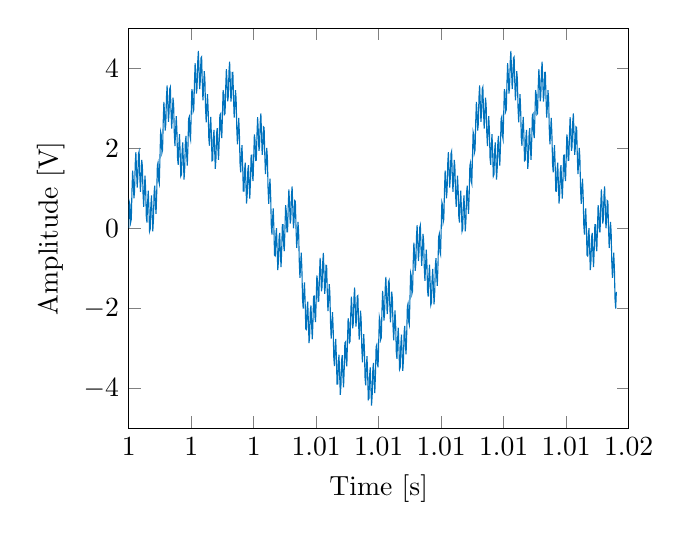
\begin{tikzpicture}

\begin{axis}[%
width=2.5in,
height=2in,
at={(0.758in,0.481in)},
scale only axis,
ylabel={Amplitude [V]},
xlabel={Time [s]},
xmin=1,
xmax=1.016,
ymin=-5,
ymax=5,
axis background/.style={fill=white}
]
\addplot [color=mycolor1,solid,forget plot]
  table[row sep=crcr]{%
1	-1.11672932546961e-12\\
1.00002083333333	0.652757892078335\\
1.00004166666667	0.587349890023828\\
1.0000625	0.146909489046233\\
1.00008333333333	0.223995166837137\\
1.00010416666667	0.934380339244883\\
1.000125	1.4424840683692\\
1.00014583333333	1.19726771883383\\
1.00016666666667	0.746598091694919\\
1.0001875	0.92293833429173\\
1.00020833333333	1.60750440295087\\
1.00022916666667	1.9048856404918\\
1.00025	1.46930339511977\\
1.00027083333333	1.01653045977608\\
1.00029166666667	1.26263240276267\\
1.0003125	1.86270388915173\\
1.00033333333333	1.92277317813085\\
1.00035416666667	1.32603612280444\\
1.000375	0.907442872755015\\
1.00039583333333	1.21781178554506\\
1.00041666666667	1.70946983720116\\
1.0004375	1.55055817255171\\
1.00045833333333	0.860865079218482\\
1.00047916666667	0.53718800400296\\
1.0005	0.927050983125387\\
1.00052083333333	1.31675511683433\\
1.00054166666667	0.992601532601192\\
1.0005625	0.302114348275203\\
1.00058333333333	0.142091146744287\\
1.00060416666667	0.632320406074452\\
1.000625	0.940943515908688\\
1.00064583333333	0.520287751415575\\
1.00066666666667	-0.0788281764465147\\
1.0006875	-0.0214537104939965\\
1.00070833333333	0.575607464134635\\
1.00072916666667	0.818384122427766\\
1.00075	0.361971499217519\\
1.00077083333333	-0.0775642135436644\\
1.00079166666667	0.215550454493061\\
1.0008125	0.895537582574299\\
1.00083333333333	1.06698729810894\\
1.00085416666667	0.611116395391016\\
1.000875	0.36038891296074\\
1.00089583333333	0.862672596186314\\
1.00091666666667	1.56692980693766\\
1.0009375	1.63758065728524\\
1.00095833333333	1.19039966567192\\
1.00097916666667	1.11794646474763\\
1.001	1.76335575687202\\
1.00102083333333	2.40846290707494\\
1.00104166666667	2.3351033321295\\
1.0010625	1.88641188970103\\
1.00108333333333	1.95494847125735\\
1.00110416666667	2.65648795750017\\
1.001125	3.15545092617692\\
1.00114583333333	2.90080030814128\\
1.00116666666667	2.44040452096744\\
1.0011875	2.60672837851411\\
1.00120833333333	3.28098955336844\\
1.00122916666667	3.56777915404332\\
1.00125	3.12132034356231\\
1.00127083333333	2.65738777850364\\
1.00129166666667	2.89204893932605\\
1.0013125	3.48040045141274\\
1.00133333333333	3.52847258210769\\
1.00135416666667	2.91946324017319\\
1.001375	2.48832467798725\\
1.00139583333333	2.78587740267449\\
1.00141666666667	3.26445058626241\\
1.0014375	3.09218761560226\\
1.00145833333333	2.38887906597711\\
1.00147916666667	2.05132471714981\\
1.0015	2.42705098312819\\
1.00152083333333	2.80236138641024\\
1.00154166666667	2.46355952076257\\
1.0015625	1.75817201395334\\
1.00158333333333	1.5829990019436\\
1.00160416666667	2.05783155865386\\
1.001625	2.35081371187642\\
1.00164583333333	1.91427541676375\\
1.00166666666667	1.29903810567761\\
1.0016875	1.34005509811438\\
1.00170833333333	1.92052551169827\\
1.00172916666667	2.14648096416106\\
1.00175	1.67301957256794\\
1.00177083333333	1.21621045007992\\
1.00179166666667	1.49183002676004\\
1.0018125	2.15410337955508\\
1.00183333333333	2.30762367103566\\
1.00185416666667	1.83361076760399\\
1.001875	1.56453181634743\\
1.00189583333333	2.04825770705887\\
1.00191666666667	2.73375398138097\\
1.0019375	2.78544396599538\\
1.00195833333333	2.31910542817288\\
1.00197916666667	2.22730128311881\\
1.002	2.85316954888403\\
1.00202083333333	3.47854893873613\\
1.00204166666667	3.38527824970577\\
1.0020625	2.91649575113081\\
1.00208333333333	2.96476477697731\\
1.00210416666667	3.64586368067738\\
1.002125	4.12421654237851\\
1.00214583333333	3.84878982437021\\
1.00216666666667	3.36745550409405\\
1.0021875	3.5126819831277\\
1.00220833333333	4.16569054898219\\
1.00222916666667	4.43107595169184\\
1.00225	3.96306502178486\\
1.00227083333333	3.47743610868781\\
1.00229166666667	3.69026041040724\\
1.0023125	4.25663829396775\\
1.00233333333333	4.28260379178242\\
1.00235416666667	3.65135860046419\\
1.002375	3.19785878238624\\
1.00239583333333	3.47292867617274\\
1.00241666666667	3.92890130615643\\
1.0024375	3.73392393167936\\
1.00245833333333	3.00779102003364\\
1.00247916666667	2.64730626179773\\
1.0025	2.99999999999949\\
1.00252083333333	3.35217970364723\\
1.00254166666667	2.99015292982671\\
1.0025625	2.26145028576494\\
1.00258333333333	2.06287590237211\\
1.00260416666667	2.51422486326038\\
1.002625	2.783645220013\\
1.00264583333333	2.32347096498735\\
1.00266666666667	1.68452758042935\\
1.0026875	1.70177244775797\\
1.00270833333333	2.25840875783057\\
1.00272916666667	2.46047221223006\\
1.00275	1.96306502178498\\
1.00277083333333	1.48226040265533\\
1.00279166666667	1.73383889640535\\
1.0028125	2.37202969929466\\
1.00283333333333	2.50143010031115\\
1.00285416666667	2.00326409868597\\
1.002875	1.71000298000577\\
1.00289583333333	2.16952177755858\\
1.00291666666667	2.83079018075887\\
1.0029375	2.85823566758721\\
1.00295833333333	2.36764015949874\\
1.00297916666667	2.25157072800749\\
1.003	2.85316954887901\\
1.00302083333333	3.4542794938477\\
1.00304166666667	3.33674351838003\\
1.0030625	2.84370404953903\\
1.00308333333333	2.86772857759868\\
1.00310416666667	3.52459961017664\\
1.003125	3.97874537872047\\
1.00314583333333	3.67913649328858\\
1.00316666666667	3.17364907481896\\
1.0031875	3.29475566339011\\
1.00320833333333	3.92368167933627\\
1.00322916666667	4.16502599911649\\
1.00325	3.67301957256481\\
1.00327083333333	3.16344486061889\\
1.00329166666667	3.35237716427433\\
1.0033125	3.89492094432336\\
1.00333333333333	3.89711431702883\\
1.00335416666667	3.24216305224085\\
1.003375	2.76502727424999\\
1.00339583333333	3.01653537156947\\
1.00341666666667	3.44902440572722\\
1.0034375	3.23064565986786\\
1.00345833333333	2.4811976109695\\
1.00347916666667	2.09748794456092\\
1.0035	2.42705098312692\\
1.00352083333333	2.75619815899852\\
1.00354166666667	2.371240975767\\
1.0035625	1.61971396968814\\
1.00358333333333	1.39842518247764\\
1.00360416666667	1.8271735897614\\
1.003625	2.07411111561397\\
1.00364583333333	1.59157560469671\\
1.00366666666667	0.930396370754758\\
1.0036875	0.925534605204918\\
1.00370833333333	1.46019728674869\\
1.00372916666667	1.64042388204629\\
1.00375	1.12132034356339\\
1.00377083333333	0.618963605007334\\
1.00379166666667	0.849137900791183\\
1.0038125	1.46607609468082\\
1.00383333333333	1.57437911718302\\
1.00385416666667	1.05527458245768\\
1.003875	0.741237363803573\\
1.00389583333333	1.18014605438358\\
1.00391666666667	1.82097387503902\\
1.0039375	1.82815180615838\\
1.00395833333333	1.31746524192355\\
1.00397916666667	1.18148469634668\\
1.004	1.76335575687482\\
1.00402083333333	2.34492467547546\\
1.00404166666667	2.20803775587563\\
1.0040625	1.6958407408285\\
1.00408333333333	1.70090440315421\\
1.00410416666667	2.33901449930376\\
1.004125	2.77460247533372\\
1.00414583333333	2.45664212107625\\
1.00416666666667	1.93301270189276\\
1.0041875	2.03618986640823\\
1.00420833333333	2.64740210706844\\
1.00422916666667	2.87125133549302\\
1.00425	2.36197149921506\\
1.00427083333333	1.83534801888732\\
1.00429166666667	2.00745911671049\\
1.0043125	2.53341213571518\\
1.00433333333333	2.51924803490577\\
1.00435416666667	1.84817538689412\\
1.004375	1.3551570782823\\
1.00439583333333	1.59102421898877\\
1.00441666666667	2.00811655052768\\
1.0044375	1.7745879941895\\
1.00445833333333	1.01023962280938\\
1.00447916666667	0.61188167498553\\
1.0045	0.927050983124141\\
1.00452083333333	1.2420614458522\\
1.00454166666667	0.843226989008768\\
1.0045625	0.0780845266354165\\
1.00458333333333	-0.156555566584843\\
1.00460416666667	0.259107972630448\\
1.004625	0.493229310380898\\
1.00464583333333	-0.00185151267107919\\
1.00466666666667	-0.675303033221497\\
1.0046875	-0.692161957056392\\
1.00470833333333	-0.169219249811889\\
1.00472916666667	-0.000433436681713584\\
1.00475	-0.530696604879047\\
1.00477083333333	-1.04392990854513\\
1.00479166666667	-0.824347249626852\\
1.0048125	-0.217713949541869\\
1.00483333333333	-0.119427312088364\\
1.00485416666667	-0.648258006851781\\
1.004875	-0.97172949400326\\
1.00489583333333	-0.541961563871422\\
1.00491666666667	0.0900205706206517\\
1.0049375	0.0886494055041014\\
1.00495833333333	-0.430288200181486\\
1.00497916666667	-0.57422031865003\\
1.005	-3.11903854464376e-12\\
1.00502083333333	0.574220318648516\\
1.00504166666667	0.430288200180768\\
1.0050625	-0.0886494055048834\\
1.00508333333333	-0.0900205706218596\\
1.00510416666667	0.541961563869971\\
1.005125	0.971729494002561\\
1.00514583333333	0.648258006851847\\
1.00516666666667	0.119427312088224\\
1.0051875	0.217713949541024\\
1.00520833333333	0.824347249626029\\
1.00522916666667	1.04392990854522\\
1.00525	0.530696604879773\\
1.00527083333333	0.000433436682068133\\
1.00529166666667	0.169219249811607\\
1.0053125	0.692161957056349\\
1.00533333333333	0.675303033222858\\
1.00535416666667	0.00185151267297182\\
1.005375	-0.493229310380118\\
1.00539583333333	-0.25910797263024\\
1.00541666666667	0.156555566585447\\
1.0054375	-0.0780845266339255\\
1.00545833333333	-0.843226989007124\\
1.00547916666667	-1.2420614458504\\
1.0055	-0.927050983123155\\
1.00552083333333	-0.611881674984052\\
1.00554166666667	-1.01023962279936\\
1.0055625	-1.77458799418801\\
1.00558333333333	-2.00811655052922\\
1.00560416666667	-1.59102421898888\\
1.005625	-1.35515707828119\\
1.00564583333333	-1.84817538689223\\
1.00566666666667	-2.51924803490486\\
1.0056875	-2.53341213571523\\
1.00570833333333	-2.00745911671077\\
1.00572916666667	-1.83534801888549\\
1.00575	-2.36197149921434\\
1.00577083333333	-2.87125133549306\\
1.00579166666667	-2.6474021070695\\
1.0058125	-2.03618986640908\\
1.00583333333333	-1.93301270189291\\
1.00585416666667	-2.45664212107619\\
1.005875	-2.77460247533443\\
1.00589583333333	-2.33901449930522\\
1.00591666666667	-1.70090440315621\\
1.0059375	-1.69584074082979\\
1.00595833333333	-2.20803775587601\\
1.00597916666667	-2.34492467547665\\
1.006	-1.76335575687652\\
1.00602083333333	-1.18148469634786\\
1.00604166666667	-1.31746524192393\\
1.0060625	-1.8281518061591\\
1.00608333333333	-1.8209738750405\\
1.00610416666667	-1.18014605438504\\
1.006125	-0.741237363804282\\
1.00614583333333	-1.05527458245788\\
1.00616666666667	-1.57437911718342\\
1.0061875	-1.46607609468193\\
1.00620833333333	-0.849137900792265\\
1.00622916666667	-0.618963605007264\\
1.00625	-1.12132034356268\\
1.00627083333333	-1.64042388204371\\
1.00629166666667	-1.46019728674898\\
1.0063125	-0.925534605204974\\
1.00633333333333	-0.930396370753864\\
1.00635416666667	-1.59157560469539\\
1.006375	-2.07411111561321\\
1.00639583333333	-1.82717358976121\\
1.00641666666667	-1.39842518247705\\
1.0064375	-1.61971396968667\\
1.00645833333333	-2.37124097576537\\
1.00647916666667	-2.75619815899763\\
1.0065	-2.42705098312653\\
1.00652083333333	-2.09748794456003\\
1.00654166666667	-2.48119761096787\\
1.0065625	-3.23064565986639\\
1.00658333333333	-3.44902440572663\\
1.00660416666667	-3.01653537156856\\
1.006625	-2.76502727424876\\
1.00664583333333	-3.24216305223953\\
1.00666666666667	-3.89711431702794\\
1.0066875	-3.89492094432342\\
1.00670833333333	-3.3523771642748\\
1.00672916666667	-3.16344486061872\\
1.00675	-3.67301957256426\\
1.00677083333333	-4.1650259991167\\
1.00679166666667	-3.92368167933735\\
1.0068125	-3.29475566339098\\
1.00683333333333	-3.17364907481926\\
1.00685416666667	-3.67913649328854\\
1.006875	-3.97874537872119\\
1.00689583333333	-3.52459961017883\\
1.00691666666667	-2.8677285776007\\
1.0069375	-2.84370404954033\\
1.00695833333333	-3.33674351838043\\
1.00697916666667	-3.4542794938489\\
1.007	-2.85316954888972\\
1.00702083333333	-2.25157072800869\\
1.00704166666667	-2.36764015950003\\
1.0070625	-2.85823566758852\\
1.00708333333333	-2.8307901807609\\
1.00710416666667	-2.16952177756006\\
1.007125	-1.7100029800065\\
1.00714583333333	-2.00326409868594\\
1.00716666666667	-2.50143010031133\\
1.0071875	-2.37202969929589\\
1.00720833333333	-1.73383889640644\\
1.00722916666667	-1.48226040265528\\
1.00725	-1.96306502178429\\
1.00727083333333	-2.46047221222979\\
1.00729166666667	-2.25840875783093\\
1.0073125	-1.70177244775809\\
1.00733333333333	-1.68452758042851\\
1.00735416666667	-2.32347096498605\\
1.007375	-2.78364522001229\\
1.00739583333333	-2.51422486326023\\
1.00741666666667	-2.06287590237157\\
1.0074375	-2.26145028576349\\
1.00745833333333	-2.9901529298251\\
1.00747916666667	-3.35217970364637\\
1.0075	-2.99999999999913\\
1.00752083333333	-2.64730626179687\\
1.00754166666667	-3.00779102002487\\
1.0075625	-3.73392393167791\\
1.00758333333333	-3.92890130615587\\
1.00760416666667	-3.47292867617258\\
1.007625	-3.1978587823855\\
1.00764583333333	-3.6513586004629\\
1.00766666666667	-4.28260379178155\\
1.0076875	-4.25663829396783\\
1.00770833333333	-3.69026041040757\\
1.00772916666667	-3.47743610868751\\
1.00775	-3.96306502178418\\
1.00777083333333	-4.43107595169181\\
1.00779166666667	-4.16569054898307\\
1.0078125	-3.51268198312859\\
1.00783333333333	-3.36745550409416\\
1.00785416666667	-3.84878982437012\\
1.007875	-4.12421654237983\\
1.00789583333333	-3.64586368067952\\
1.00791666666667	-2.96476477697848\\
1.0079375	-2.91649575113121\\
1.00795833333333	-3.38527824970611\\
1.00797916666667	-3.47854893873725\\
1.008	-2.85316954888578\\
1.00802083333333	-2.22730128312094\\
1.00804166666667	-2.31910542817419\\
1.0080625	-2.78544396599672\\
1.00808333333333	-2.73375398138223\\
1.00810416666667	-2.04825770706038\\
1.008125	-1.56453181634818\\
1.00814583333333	-1.83361076760398\\
1.00816666666667	-2.30762367103631\\
1.0081875	-2.15410337955633\\
1.00820833333333	-1.49183002676116\\
1.00822916666667	-1.2162104500799\\
1.00825	-1.67301957256727\\
1.00827083333333	-2.14648096415881\\
1.00829166666667	-1.92052551169861\\
1.0083125	-1.34005509811413\\
1.00833333333333	-1.29903810567631\\
1.00835416666667	-1.91427541676192\\
1.008375	-2.3508137118757\\
1.00839583333333	-2.05783155865353\\
1.00841666666667	-1.58299900194288\\
1.0084375	-1.75817201395172\\
1.00845833333333	-2.46355952076011\\
1.00847916666667	-2.8023613864083\\
1.0085	-2.42705098312675\\
1.00852083333333	-2.05132471714877\\
1.00854166666667	-2.38887906597533\\
1.0085625	-3.09218761560083\\
1.00858333333333	-3.26445058626187\\
1.00860416666667	-2.78587740267435\\
1.008625	-2.48832467798653\\
1.00864583333333	-2.91946324017136\\
1.00866666666667	-3.52847258210685\\
1.0086875	-3.48040045141286\\
1.00870833333333	-2.8920489393264\\
1.00872916666667	-2.65738777850335\\
1.00875	-3.12132034356165\\
1.00877083333333	-3.5677791540433\\
1.00879166666667	-3.28098955336933\\
1.0088125	-2.60672837852076\\
1.00883333333333	-2.44040452096765\\
1.00885416666667	-2.90080030814129\\
1.008875	-3.15545092617769\\
1.00889583333333	-2.6564879575017\\
1.00891666666667	-1.95494847125863\\
1.0089375	-1.88641188970154\\
1.00895833333333	-2.33510333212968\\
1.00897916666667	-2.40846290707591\\
1.009	-1.76335575688224\\
1.00902083333333	-1.11794646474888\\
1.00904166666667	-1.19039966567209\\
1.0090625	-1.63758065728547\\
1.00908333333333	-1.56692980693866\\
1.00910416666667	-0.862672596187553\\
1.009125	-0.360388912961516\\
1.00914583333333	-0.611116395391027\\
1.00916666666667	-1.06698729810961\\
1.0091875	-0.895537582574923\\
1.00920833333333	-0.215550454493962\\
1.00922916666667	0.077564213543669\\
1.00925	-0.361971499216871\\
1.00927083333333	-0.818384122427489\\
1.00929166666667	-0.575607464134759\\
1.0093125	0.0214537104942232\\
1.00933333333333	0.0788281764477978\\
1.00935416666667	-0.520287751414314\\
1.009375	-0.940943515907986\\
1.00939583333333	-0.632320406074322\\
1.00941666666667	-0.142091146743762\\
1.0094375	-0.30211434827295\\
1.00945833333333	-0.992601532598748\\
1.00947916666667	-1.31675511683261\\
1.0095	-0.927050983125064\\
1.00952083333333	-0.53718800400214\\
1.00954166666667	-0.860865079209187\\
1.0095625	-1.55055817255029\\
1.00958333333333	-1.70946983719985\\
1.00960416666667	-1.21781178554388\\
1.009625	-0.90744287275334\\
1.00964583333333	-1.32603612280285\\
1.00966666666667	-1.92277317812969\\
1.0096875	-1.86270388915185\\
1.00970833333333	-1.26263240276303\\
1.00972916666667	-1.01653045977535\\
1.00975	-1.46930339511879\\
1.00977083333333	-1.90488564049192\\
1.00979166666667	-1.60750440295178\\
1.0098125	-0.922938334292656\\
1.00983333333333	-0.74659809169514\\
1.00985416666667	-1.19726771883385\\
1.009875	-1.44248406836998\\
1.00989583333333	-0.934380339246416\\
1.00991666666667	-0.223995166839215\\
1.0099375	-0.146909489046756\\
1.00995833333333	-0.587349890024286\\
1.00997916666667	-0.652757892079591\\
1.01	-6.56096242179594e-13\\
1.01002083333333	0.652757892078581\\
1.01004166666667	0.587349890023746\\
1.0100625	0.146909489046187\\
1.01008333333333	0.223995166832657\\
1.01010416666667	0.934380339245285\\
1.010125	1.4424840683693\\
1.01014583333333	1.19726771883364\\
1.01016666666667	0.74659809169517\\
1.0101875	0.922938334292299\\
1.01020833333333	1.60750440295146\\
1.01022916666667	1.90488564049203\\
1.01025	1.46930339511942\\
1.01027083333333	1.01653045977758\\
1.01029166666667	1.26263240276312\\
1.0103125	1.86270388915211\\
1.01033333333333	1.92277317813052\\
1.01035416666667	1.32603612280396\\
1.010375	0.907442872754783\\
1.01039583333333	1.21781178554508\\
1.01041666666667	1.70946983720103\\
1.0104375	1.55055817255206\\
1.01045833333333	0.860865079217942\\
1.01047916666667	0.537188004002735\\
1.0105	0.927050983125372\\
1.01052083333333	1.31675511683411\\
1.01054166666667	0.992601532600652\\
1.0105625	0.302114348274719\\
1.01058333333333	0.142091146744951\\
1.01060416666667	0.6323204060752\\
1.010625	0.940943515908459\\
1.01064583333333	0.520287751415093\\
1.01066666666667	-0.0788281764468367\\
1.0106875	-0.0214537104939442\\
1.01070833333333	0.575607464134762\\
1.01072916666667	0.818384122427721\\
1.01075	0.361971499217479\\
1.01077083333333	-0.0775642135434629\\
1.01079166666667	0.215550454493614\\
1.0108125	0.895537582568398\\
1.01083333333333	1.06698729810915\\
1.01085416666667	0.611116395390569\\
1.010875	0.360388912960502\\
1.01089583333333	0.862672596186004\\
1.01091666666667	1.56692980693796\\
1.0109375	1.6375806572852\\
1.01095833333333	1.19039966567185\\
1.01097916666667	1.11794646474789\\
1.011	1.76335575687158\\
1.01102083333333	2.40846290707429\\
1.01104166666667	2.33510333212855\\
1.0110625	1.886411889701\\
1.01108333333333	1.95494847125765\\
1.01110416666667	2.65648795750059\\
1.011125	3.15545092617704\\
1.01114583333333	2.9008003081411\\
1.01116666666667	2.44040452096737\\
1.0111875	2.606728378514\\
1.01120833333333	3.2809895533687\\
1.01122916666667	3.56777915404323\\
1.01125	3.12132034356198\\
1.01127083333333	2.65738777850349\\
1.01129166666667	2.89204893932619\\
1.0113125	3.48040045141304\\
1.01133333333333	3.52847258210761\\
1.01135416666667	2.91946324017295\\
1.011375	2.48832467798726\\
1.01139583333333	2.78587740267476\\
1.01141666666667	3.26445058626252\\
1.0114375	3.09218761560201\\
1.01145833333333	2.38887906597659\\
1.01147916666667	2.05132471714961\\
1.0115	2.4270509831282\\
1.01152083333333	2.80236138641004\\
1.01154166666667	2.46355952076904\\
1.0115625	1.75817201395288\\
1.01158333333333	1.5829990019435\\
1.01160416666667	2.05783155865391\\
1.011625	2.35081371187622\\
1.01164583333333	1.91427541676329\\
1.01166666666667	1.29903810567732\\
1.0116875	1.34005509811445\\
1.01170833333333	1.92052551169866\\
1.01172916666667	2.14648096416093\\
1.01175	1.67301957256763\\
1.01177083333333	1.21621045007985\\
1.01179166666667	1.49183002676032\\
1.0118125	2.15410337955535\\
1.01183333333333	2.30762367103561\\
1.01185416666667	1.83361076760328\\
1.011875	1.56453181634706\\
1.01189583333333	2.04825770705872\\
1.01191666666667	2.73375398138129\\
1.0119375	2.7854439659955\\
1.01195833333333	2.31910542817295\\
1.01197916666667	2.22730128311921\\
1.012	2.85316954888373\\
1.01202083333333	3.47854893873552\\
1.01204166666667	3.38527824970574\\
1.0120625	2.91649575113081\\
1.01208333333333	2.96476477697234\\
1.01210416666667	3.64586368067783\\
1.012125	4.12421654237867\\
1.01214583333333	3.84878982436951\\
1.01216666666667	3.36745550409355\\
1.0121875	3.51268198312798\\
1.01220833333333	4.16569054898249\\
1.01222916666667	4.43107595169179\\
1.01225	3.96306502178457\\
1.01227083333333	3.47743610868977\\
1.01229166666667	3.69026041040766\\
1.0123125	4.2566382939682\\
1.01233333333333	4.28260379178215\\
1.01235416666667	3.65135860046377\\
1.012375	3.19785878238607\\
1.01239583333333	3.47292867617283\\
1.01241666666667	3.92890130615636\\
1.0124375	3.73392393167895\\
1.01245833333333	3.00779102003404\\
1.01247916666667	2.64730626179757\\
1.0125	2.99999999999953\\
1.01252083333333	3.35217970364706\\
1.01254166666667	2.99015292982622\\
1.0125625	2.2614502857645\\
1.01258333333333	2.06287590237205\\
1.01260416666667	2.51422486326047\\
1.012625	2.78364522001284\\
1.01264583333333	2.3234709649869\\
1.01266666666667	1.68452758042909\\
1.0126875	1.70177244775809\\
1.01270833333333	2.25840875783076\\
1.01272916666667	2.46047221222996\\
1.01275	1.9630650217847\\
1.01277083333333	1.4822604026553\\
1.01279166666667	1.73383889640567\\
1.0128125	2.37202969928954\\
1.01283333333333	2.50143010031114\\
1.01285416666667	2.00326409868585\\
1.012875	1.71000298000595\\
1.01289583333333	2.16952177755906\\
1.01291666666667	2.83079018075924\\
1.0129375	2.85823566758725\\
1.01295833333333	2.36764015949874\\
1.01297916666667	2.25157072800691\\
1.013	2.85316954887955\\
1.01302083333333	3.45427949384803\\
1.01304166666667	3.33674351838004\\
1.0130625	2.84370404953907\\
1.01308333333333	2.86772857759893\\
1.01310416666667	3.524599610177\\
1.013125	3.97874537871989\\
1.01314583333333	3.67913649328779\\
1.01316666666667	3.1736490748185\\
1.0131875	3.29475566339029\\
1.01320833333333	3.92368167933646\\
1.01322916666667	4.16502599911647\\
1.01325	3.67301957256455\\
1.01327083333333	3.16344486061894\\
1.01329166666667	3.35237716427479\\
1.0133125	3.89492094432385\\
1.01333333333333	3.8971143170286\\
1.01335416666667	3.24216305224046\\
1.013375	2.76502727424985\\
1.01339583333333	3.01653537156959\\
1.01341666666667	3.44902440572797\\
1.0134375	3.23064565986831\\
1.01345833333333	2.48119761096994\\
1.01347916666667	2.09748794456079\\
1.0135	2.427050983127\\
1.01352083333333	2.75619815899839\\
1.01354166666667	2.37124097577483\\
1.0135625	1.6197139696886\\
1.01358333333333	1.3984251824784\\
1.01360416666667	1.82717358976153\\
1.013625	2.07411111561384\\
1.01364583333333	1.59157560469611\\
1.01366666666667	0.93039637075431\\
1.0136875	0.925534605204841\\
1.01370833333333	1.46019728674869\\
1.01372916666667	1.64042388204611\\
1.01375	1.12132034356291\\
1.01377083333333	0.618963605007093\\
1.01379166666667	0.84913790079154\\
1.0138125	1.46607609468116\\
1.01383333333333	1.57437911718304\\
1.01385416666667	1.0552745824576\\
1.013875	0.741237363803791\\
1.01389583333333	1.1801460543841\\
1.01391666666667	1.82097387503942\\
1.0139375	1.82815180615845\\
1.01395833333333	1.31746524192358\\
1.01397916666667	1.18148469634704\\
1.014	1.7633557568754\\
1.01402083333333	2.34492467547583\\
1.01404166666667	2.20803775587567\\
1.0140625	1.69584074082857\\
1.01408333333333	1.70090440315047\\
1.01410416666667	2.33901449930428\\
1.014125	2.77460247533395\\
1.01414583333333	2.45664212107617\\
1.01416666666667	1.93301270189279\\
1.0141875	2.03618986640858\\
1.01420833333333	2.6474021070685\\
1.01422916666667	2.87125133549273\\
1.01425	2.36197149921453\\
1.01427083333333	1.83534801888728\\
1.01429166666667	2.00745911671042\\
1.0143125	2.53341213571504\\
1.01433333333333	2.51924803490525\\
1.01435416666667	1.84817538689344\\
1.014375	1.35515707828219\\
1.01439583333333	1.59102421898964\\
1.01441666666667	2.00811655052846\\
1.0144375	1.77458799418998\\
1.01445833333333	1.01023962280897\\
1.01447916666667	0.611881674985429\\
1.0145	0.927050983124249\\
1.01452083333333	1.2420614458521\\
1.01454166666667	0.843226989009229\\
1.0145625	0.0780845266358958\\
1.01458333333333	-0.156555566584057\\
1.01460416666667	0.259107972630598\\
1.014625	0.493229310380792\\
1.01464583333333	-0.00185151267143813\\
1.01466666666667	-0.675303033221697\\
1.0146875	-0.69216195705587\\
1.01470833333333	-0.169219249811404\\
1.01472916666667	-0.000433436681636479\\
1.01475	-0.530696604879269\\
1.01477083333333	-1.04392990854545\\
1.01479166666667	-0.824347249626816\\
1.0148125	-0.217713949547013\\
1.01483333333333	-0.119427312088778\\
1.01485416666667	-0.648258006852741\\
1.014875	-0.97172949400401\\
1.01489583333333	-0.541961563871231\\
1.01491666666667	0.090020570620726\\
1.0149375	0.0886494055041845\\
1.01495833333333	-0.430288200181438\\
1.01497916666667	-0.574220318649655\\
1.015	-3.43853289453089e-12\\
1.01502083333333	0.57422031864799\\
1.01504166666667	0.430288200180816\\
1.0150625	-0.0886494055048002\\
1.01508333333333	-0.0900205706214449\\
1.01510416666667	0.541961563870501\\
1.015125	0.971729494002795\\
1.01514583333333	0.64825800685178\\
1.01516666666667	0.119427312088265\\
1.0151875	0.217713949541383\\
1.01520833333333	0.824347249626403\\
1.01522916666667	1.04392990854524\\
1.01525	0.53069660487955\\
1.01527083333333	0.000433436682026611\\
1.01529166666667	0.169219249811856\\
1.0153125	0.692161957056523\\
1.01533333333333	0.675303033222325\\
1.01535416666667	0.00185151268052736\\
1.015375	-0.493229310380224\\
1.01539583333333	-0.259107972630091\\
1.01541666666667	0.156555566585116\\
1.0154375	-0.078084526634615\\
1.01545833333333	-0.843226989007868\\
1.01547916666667	-1.24206144585082\\
1.0155	-0.927050983123046\\
1.01552083333333	-0.611881674984154\\
1.01554166666667	-1.0102396228001\\
1.0155625	-1.7745879941887\\
1.01558333333333	-2.00811655052922\\
1.01560416666667	-1.59102421898874\\
};
\end{axis}
\end{tikzpicture}%
		\caption{An AM modulated sine with a 100 Hz, 1 $k$Hz and 10 $k$Hz tone.}
		\label{fig:Signal01k1k10k}
	\end{subfigure}
	\hfill
	\begin{subfigure}[b]{0.45\textwidth}
		\centering
			\tikzsetnextfilename{OctFilter01k1k10k}
			% This file was created by matlab2tikz.
%
%The latest updates can be retrieved from
%  http://www.mathworks.com/matlabcentral/fileexchange/22022-matlab2tikz-matlab2tikz
%where you can also make suggestions and rate matlab2tikz.
%
\definecolor{mycolor1}{rgb}{0.00000,0.44700,0.74100}%
%
\begin{tikzpicture}

\begin{axis}[%
width=2.5in,
height=2in,
scale only axis,
xmode=log,
ylabel={Amplitude [dB]},
xlabel={Frequency [Hz]},
xmin=20,
xmax=2e+04,
xminorticks=true,
ymin=-1,
ymax=3,
axis background/.style={fill=white}
]
\addplot[const plot,color=MATLABred,solid,forget plot] plot table[row sep=crcr] {%
21.9	0.0182\\
27.5	0.0212\\
34.7	0.0255\\
43.6	0.0323\\
54.9	0.0462\\
69.1	0.16\\
87.1	2.08\\
110	0.15\\
138	0.0285\\
174	0.0145\\
219	0.00813\\
275	0.00441\\
347	0.00189\\
436	0.000836\\
549	0.00369\\
691	0.0438\\
871	0.706\\
1.1e+03	0.044\\
1.38e+03	0.00419\\
1.74e+03	0.0019\\
2.19e+03	0.00109\\
2.75e+03	0.000605\\
3.47e+03	0.000272\\
4.36e+03	0.000159\\
5.49e+03	0.000926\\
6.91e+03	0.018\\
8.71e+03	0.353\\
1.1e+04	0.0286\\
1.38e+04	0.00322\\
1.79e+04	0.00162\\
};
\end{axis}
\end{tikzpicture}%
		\caption{The output from the signal shown in figure \ref{fig:Signal01k1k10k}.}
		\label{fig:OctFilter01k1k10k}
	\end{subfigure}	
	\begin{subfigure}[b]{0.45\textwidth}
		\centering
			\tikzsetnextfilename{PinkNoise5sec}
			% This file was created by matlab2tikz.
%
%The latest updates can be retrieved from
%  http://www.mathworks.com/matlabcentral/fileexchange/22022-matlab2tikz-matlab2tikz
%where you can also make suggestions and rate matlab2tikz.
%
\definecolor{mycolor1}{rgb}{0.00000,0.44700,0.74100}%
%
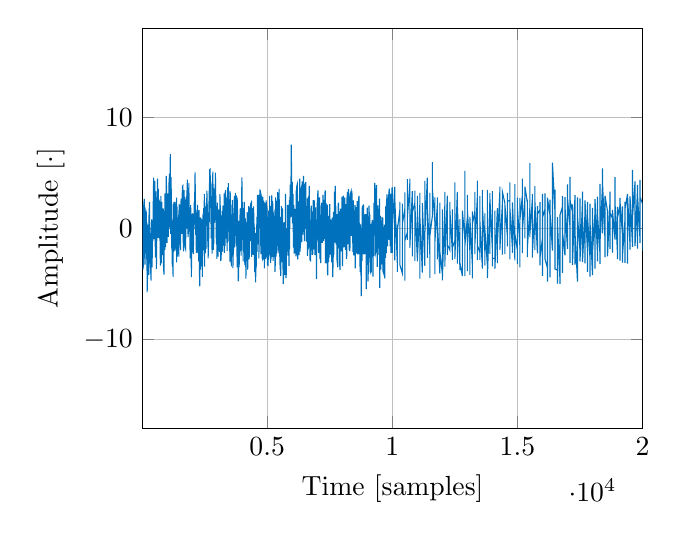
\begin{tikzpicture}

\begin{axis}[%
width=2.5in,
height=2in,
scale only axis,
%xmode=log,
ylabel={Amplitude [$\cdot$]},
xlabel={Time [samples]},
xmin=20,
xmax=2e+04,
xminorticks=true,
%xtick={0,4000,...,20000},
%xticklabels={0,1,2,3,4,5},
ymin=-18,
ymax=18,
xmajorgrids,
xminorgrids,
ymajorgrids,
yminorgrids,
axis background/.style={fill=white}
]
\addplot [color=mycolor1,solid,forget plot]
  table[row sep=crcr]{%
19	-0.0964\\
35	2.11\\
45	-3.7\\
59	-0.925\\
63	1.7\\
86	2.63\\
90	-1.57\\
120	-3.27\\
125	-0.196\\
129	-1.77\\
150	1.59\\
174	1.38\\
181	-2.81\\
191	0.516\\
204	-5.74\\
217	-4.44\\
236	0.325\\
238	-0.785\\
254	-4.16\\
268	-4.15\\
272	0.717\\
300	2.37\\
308	-3.18\\
323	-0.435\\
332	-3.13\\
362	-4.72\\
369	-0.014\\
385	0.784\\
400	-3.52\\
400	-3.52\\
427	0.521\\
429	-1.13\\
454	3.13\\
464	4.55\\
477	-0.987\\
491	-0.62\\
497	4.21\\
510	4.19\\
533	-2.63\\
546	3.32\\
562	-1.23\\
575	-3.67\\
581	2.78\\
593	-1.14\\
618	4.37\\
622	4.46\\
641	-0.864\\
648	3.53\\
671	-0.755\\
678	-0.783\\
682	2.48\\
703	2.33\\
721	-1.45\\
734	-3.37\\
752	2.9\\
753	2.09\\
769	-3.17\\
787	2.38\\
788	-0.621\\
813	-2.41\\
833	0.812\\
845	1.78\\
858	-3.46\\
876	-4.17\\
883	1.57\\
909	-1.95\\
916	3.13\\
931	2.1\\
939	-1.69\\
946	-0.763\\
968	4.71\\
975	3.87\\
997	-1.31\\
1e+03	-0.924\\
1.01e+03	2.39\\
1.04e+03	3.14\\
1.05e+03	-0.777\\
1.05e+03	-0.629\\
1.08e+03	4.25\\
1.08e+03	-0.081\\
1.09e+03	4.92\\
1.11e+03	0.513\\
1.13e+03	6.67\\
1.14e+03	-0.516\\
1.16e+03	4.59\\
1.16e+03	4.59\\
1.19e+03	-1.98\\
1.19e+03	2.2\\
1.21e+03	-3.46\\
1.22e+03	0.174\\
1.24e+03	-4.38\\
1.24e+03	-2.15\\
1.27e+03	2.35\\
1.27e+03	1.85\\
1.28e+03	-2\\
1.3e+03	-1.93\\
1.32e+03	2.4\\
1.33e+03	2.05\\
1.35e+03	-1.63\\
1.37e+03	-2.08\\
1.38e+03	2.75\\
1.38e+03	-3.08\\
1.4e+03	1.94\\
1.41e+03	-2.56\\
1.41e+03	0.964\\
1.44e+03	-2.33\\
1.46e+03	1.2\\
1.47e+03	-2.56\\
1.48e+03	2.19\\
1.49e+03	-1.48\\
1.5e+03	2.09\\
1.52e+03	1.6\\
1.54e+03	-1.98\\
1.54e+03	-0.452\\
1.56e+03	2.66\\
1.58e+03	2.03\\
1.59e+03	-0.502\\
1.6e+03	-0.0871\\
1.61e+03	3.75\\
1.63e+03	3.82\\
1.64e+03	-0.715\\
1.66e+03	-2.09\\
1.68e+03	3.12\\
1.68e+03	3.43\\
1.7e+03	-1.62\\
1.71e+03	2.83\\
1.72e+03	-1.69\\
1.74e+03	-1.86\\
1.76e+03	2.6\\
1.78e+03	-0.0303\\
1.79e+03	3.4\\
1.79e+03	0.761\\
1.81e+03	4.37\\
1.81e+03	4.37\\
1.84e+03	-0.796\\
1.85e+03	-0.119\\
1.87e+03	2.89\\
1.87e+03	4.05\\
1.89e+03	-0.312\\
1.91e+03	1.88\\
1.92e+03	-2.72\\
1.92e+03	-2.72\\
1.94e+03	2.08\\
1.96e+03	0.776\\
1.97e+03	-4.39\\
1.98e+03	-2.83\\
1.99e+03	1.28\\
2.01e+03	-2.18\\
2.02e+03	1.27\\
2.04e+03	1.24\\
2.05e+03	-2.33\\
2.06e+03	-0.481\\
2.09e+03	2.46\\
2.1e+03	0.334\\
2.11e+03	3.96\\
2.12e+03	5.03\\
2.14e+03	-0.601\\
2.14e+03	2.22\\
2.17e+03	-2.22\\
2.17e+03	-2.22\\
2.17e+03	1.43\\
2.2e+03	-2.2\\
2.22e+03	2.1\\
2.23e+03	-1.6\\
2.23e+03	1.59\\
2.25e+03	0.426\\
2.26e+03	-2.98\\
2.28e+03	1.62\\
2.3e+03	-5.06\\
2.31e+03	-5.22\\
2.32e+03	0.32\\
2.33e+03	0.981\\
2.34e+03	-3.72\\
2.36e+03	0.888\\
2.39e+03	-3.43\\
2.4e+03	0.79\\
2.41e+03	-4.38\\
2.43e+03	1.22\\
2.43e+03	-2.47\\
2.46e+03	1.8\\
2.46e+03	-1.98\\
2.47e+03	-1.84\\
2.49e+03	3.06\\
2.5e+03	-3.45\\
2.51e+03	1.66\\
2.53e+03	-2.25\\
2.54e+03	1.96\\
2.56e+03	-1.86\\
2.56e+03	2.31\\
2.58e+03	0.534\\
2.59e+03	3.39\\
2.6e+03	2.62\\
2.63e+03	-1.5\\
2.63e+03	1.42\\
2.64e+03	-2.71\\
2.67e+03	-0.434\\
2.68e+03	3.37\\
2.69e+03	0.544\\
2.7e+03	5.26\\
2.72e+03	5.31\\
2.74e+03	1.8\\
2.75e+03	4.19\\
2.76e+03	-0.911\\
2.78e+03	2.89\\
2.79e+03	-0.802\\
2.8e+03	-2.29\\
2.81e+03	3.3\\
2.83e+03	5.09\\
2.85e+03	-1.94\\
2.86e+03	3.63\\
2.87e+03	-1.43\\
2.87e+03	-0.0249\\
2.88e+03	3\\
2.9e+03	0.482\\
2.92e+03	3.96\\
2.93e+03	1.58\\
2.93e+03	5.01\\
2.97e+03	-1.3\\
2.98e+03	1.98\\
2.99e+03	-2.76\\
3.01e+03	2.18\\
3.01e+03	2.3\\
3.04e+03	-2.56\\
3.04e+03	-2.56\\
3.04e+03	1.05\\
3.07e+03	1.67\\
3.09e+03	-1.75\\
3.1e+03	-2.12\\
3.11e+03	3.06\\
3.13e+03	1.47\\
3.14e+03	-2.96\\
3.16e+03	-2.73\\
3.16e+03	1.16\\
3.17e+03	-2.4\\
3.2e+03	1.32\\
3.2e+03	1.55\\
3.22e+03	-2.11\\
3.23e+03	2.04\\
3.24e+03	-1.56\\
3.27e+03	-1.19\\
3.28e+03	3.11\\
3.29e+03	-2.21\\
3.31e+03	2.53\\
3.32e+03	-1.62\\
3.32e+03	3.14\\
3.34e+03	3.43\\
3.36e+03	-0.451\\
3.37e+03	-0.94\\
3.38e+03	2.72\\
3.4e+03	-2.05\\
3.42e+03	3.68\\
3.43e+03	-0.304\\
3.45e+03	4.06\\
3.45e+03	4.06\\
3.47e+03	-0.952\\
3.48e+03	-1.23\\
3.49e+03	2.61\\
3.51e+03	-3\\
3.52e+03	3.32\\
3.53e+03	2.66\\
3.55e+03	-1.65\\
3.57e+03	-3.43\\
3.58e+03	1.24\\
3.6e+03	-2.55\\
3.6e+03	1.24\\
3.61e+03	2.52\\
3.63e+03	-3.58\\
3.65e+03	-1.62\\
3.65e+03	0.849\\
3.66e+03	-2.06\\
3.68e+03	2.04\\
3.69e+03	2.9\\
3.7e+03	-1.73\\
3.73e+03	3.17\\
3.74e+03	-0.689\\
3.77e+03	2.96\\
3.77e+03	-1.61\\
3.78e+03	1.9\\
3.8e+03	-3.52\\
3.8e+03	-1.82\\
3.8e+03	2.77\\
3.83e+03	-0.077\\
3.84e+03	-4.78\\
3.86e+03	-4.36\\
3.87e+03	0.663\\
3.88e+03	-3.5\\
3.91e+03	0.243\\
3.92e+03	1.77\\
3.93e+03	-2.08\\
3.95e+03	1.84\\
3.96e+03	-2.33\\
3.96e+03	-2.47\\
3.99e+03	4.58\\
4e+03	2.53\\
4.01e+03	-1.07\\
4.02e+03	2.34\\
4.04e+03	-2.99\\
4.05e+03	1.32\\
4.06e+03	-1.93\\
4.09e+03	2.36\\
4.1e+03	-2.77\\
4.11e+03	-3.31\\
4.12e+03	0.456\\
4.13e+03	0.881\\
4.15e+03	-4.54\\
4.18e+03	0.536\\
4.18e+03	-2.97\\
4.18e+03	-2.84\\
4.2e+03	1.45\\
4.21e+03	1.19\\
4.22e+03	-3.73\\
4.24e+03	-2.19\\
4.26e+03	1.99\\
4.27e+03	1.29\\
4.28e+03	-2.81\\
4.29e+03	-1.58\\
4.29e+03	1.88\\
4.32e+03	-1.17\\
4.33e+03	2.1\\
4.36e+03	2.29\\
4.37e+03	-2.31\\
4.38e+03	2.41\\
4.38e+03	-2.57\\
4.41e+03	1.8\\
4.42e+03	-1.14\\
4.42e+03	1.23\\
4.44e+03	-2.39\\
4.46e+03	1.96\\
4.47e+03	-2.16\\
4.48e+03	0.437\\
4.5e+03	-3.94\\
4.53e+03	-0.416\\
4.53e+03	-3.75\\
4.54e+03	-4.87\\
4.55e+03	-1.19\\
4.56e+03	-3.64\\
4.59e+03	1.01\\
4.6e+03	-2.13\\
4.61e+03	3\\
4.63e+03	2.73\\
4.64e+03	-1.43\\
4.65e+03	-0.583\\
4.66e+03	3.01\\
4.67e+03	-2.72\\
4.68e+03	1.76\\
4.7e+03	0.232\\
4.71e+03	3.5\\
4.72e+03	2.54\\
4.75e+03	-2.34\\
4.75e+03	-1.35\\
4.76e+03	2.95\\
4.8e+03	2.51\\
4.8e+03	-2.67\\
4.81e+03	-2.74\\
4.82e+03	2.85\\
4.83e+03	2.31\\
4.85e+03	-2.83\\
4.86e+03	2.49\\
4.89e+03	-0.966\\
4.89e+03	-3.61\\
4.9e+03	2.3\\
4.92e+03	0.983\\
4.94e+03	-2.76\\
4.94e+03	-1.13\\
4.96e+03	2.5\\
4.99e+03	-2.63\\
4.99e+03	2.02\\
4.99e+03	2.02\\
5.01e+03	-3.29\\
5.04e+03	-3.34\\
5.04e+03	1.01\\
5.05e+03	-2.85\\
5.06e+03	1.58\\
5.08e+03	-2.38\\
5.1e+03	2.91\\
5.1e+03	2.22\\
5.12e+03	-2.47\\
5.14e+03	-3.11\\
5.16e+03	1.99\\
5.16e+03	-2.75\\
5.18e+03	2.96\\
5.2e+03	2.04\\
5.21e+03	-2.57\\
5.22e+03	2.43\\
5.24e+03	-2.93\\
5.24e+03	-1.87\\
5.24e+03	0.909\\
5.28e+03	1.34\\
5.29e+03	-2.6\\
5.3e+03	0.0144\\
5.31e+03	-3.93\\
5.32e+03	-3.58\\
5.34e+03	2.78\\
5.36e+03	-2.56\\
5.37e+03	2.45\\
5.39e+03	1.45\\
5.39e+03	-1.6\\
5.42e+03	3.25\\
5.42e+03	-1.38\\
5.44e+03	-2.24\\
5.45e+03	3.16\\
5.46e+03	-1.02\\
5.48e+03	3.53\\
5.48e+03	2.7\\
5.5e+03	-2.21\\
5.52e+03	-3.73\\
5.53e+03	1.03\\
5.54e+03	-4.3\\
5.57e+03	1.99\\
5.57e+03	1.99\\
5.59e+03	-1.8\\
5.6e+03	-3.06\\
5.61e+03	1.79\\
5.62e+03	-0.235\\
5.64e+03	-5.02\\
5.65e+03	-4.57\\
5.67e+03	0.47\\
5.68e+03	0.477\\
5.69e+03	-4.06\\
5.7e+03	-4.19\\
5.73e+03	0.742\\
5.73e+03	3.08\\
5.75e+03	-4.5\\
5.76e+03	-4.23\\
5.78e+03	-0.0149\\
5.8e+03	-1.77\\
5.81e+03	2.05\\
5.81e+03	2.11\\
5.83e+03	-2.47\\
5.85e+03	-1.9\\
5.86e+03	2.1\\
5.87e+03	-3.39\\
5.89e+03	2.53\\
5.89e+03	-1.91\\
5.92e+03	3.92\\
5.92e+03	3.92\\
5.93e+03	0.975\\
5.95e+03	2.59\\
5.96e+03	7.52\\
5.97e+03	5.96\\
5.98e+03	1.04\\
6e+03	4.18\\
6.01e+03	0.444\\
6.03e+03	3.09\\
6.05e+03	-1.75\\
6.06e+03	2.1\\
6.08e+03	-2.29\\
6.08e+03	1.45\\
6.11e+03	-2.08\\
6.12e+03	1.73\\
6.13e+03	-1.5\\
6.15e+03	-2.54\\
6.16e+03	3.41\\
6.17e+03	-0.0846\\
6.18e+03	3.73\\
6.2e+03	3.94\\
6.21e+03	-2.13\\
6.22e+03	-2.8\\
6.23e+03	2.41\\
6.25e+03	1.24\\
6.27e+03	-2.43\\
6.27e+03	-2.43\\
6.3e+03	4.47\\
6.3e+03	1.9\\
6.31e+03	-2.11\\
6.33e+03	-1.43\\
6.35e+03	3.46\\
6.37e+03	3.67\\
6.38e+03	-1.26\\
6.39e+03	-0.116\\
6.4e+03	4.22\\
6.41e+03	3.15\\
6.42e+03	-0.584\\
6.44e+03	-0.103\\
6.45e+03	4.72\\
6.46e+03	3.86\\
6.49e+03	-1.15\\
6.49e+03	-0.543\\
6.51e+03	4.02\\
6.52e+03	-0.0668\\
6.54e+03	4.15\\
6.55e+03	2.58\\
6.57e+03	-1.11\\
6.59e+03	-1.06\\
6.6e+03	2\\
6.61e+03	-2.5\\
6.62e+03	2.63\\
6.63e+03	2.68\\
6.63e+03	-1.9\\
6.66e+03	-1.66\\
6.68e+03	3.81\\
6.68e+03	3.81\\
6.71e+03	-2.84\\
6.73e+03	-2.9\\
6.73e+03	0.73\\
6.74e+03	-1.89\\
6.76e+03	2.04\\
6.77e+03	1.48\\
6.79e+03	-1.77\\
6.8e+03	-2.4\\
6.82e+03	1.48\\
6.82e+03	-2.33\\
6.84e+03	2.52\\
6.86e+03	2.19\\
6.87e+03	-1.9\\
6.88e+03	2.51\\
6.9e+03	-0.632\\
6.9e+03	1.49\\
6.91e+03	-2.41\\
6.93e+03	1.88\\
6.95e+03	-1.51\\
6.96e+03	0.526\\
6.97e+03	-4.57\\
6.98e+03	-1.78\\
7e+03	2.13\\
7.03e+03	3.4\\
7.03e+03	-1.03\\
7.03e+03	2.1\\
7.06e+03	-2.23\\
7.06e+03	-0.99\\
7.08e+03	2.05\\
7.09e+03	2.78\\
7.11e+03	-2.77\\
7.12e+03	1.23\\
7.13e+03	-2.32\\
7.14e+03	-3.13\\
7.16e+03	1.96\\
7.18e+03	2.29\\
7.18e+03	-0.489\\
7.2e+03	2.11\\
7.2e+03	-1.31\\
7.23e+03	3.01\\
7.25e+03	-1.16\\
7.25e+03	-1.16\\
7.27e+03	2.54\\
7.29e+03	-0.968\\
7.31e+03	3.18\\
7.32e+03	3.4\\
7.33e+03	-2.21\\
7.33e+03	-3.15\\
7.35e+03	2.25\\
7.36e+03	1.78\\
7.37e+03	-3.16\\
7.4e+03	2.12\\
7.41e+03	-3.91\\
7.42e+03	-4.25\\
7.44e+03	1.12\\
7.45e+03	-3.06\\
7.47e+03	0.851\\
7.47e+03	-2.64\\
7.48e+03	0.683\\
7.5e+03	2.16\\
7.51e+03	-2.38\\
7.53e+03	0.792\\
7.53e+03	-2.1\\
7.56e+03	0.717\\
7.57e+03	-2.41\\
7.58e+03	-3.07\\
7.6e+03	0.961\\
7.61e+03	-0.603\\
7.62e+03	-4.4\\
7.64e+03	-2.46\\
7.65e+03	1.47\\
7.66e+03	-2.37\\
7.69e+03	2.03\\
7.69e+03	3.29\\
7.7e+03	-1.3\\
7.72e+03	3.8\\
7.74e+03	-0.474\\
7.74e+03	1.97\\
7.76e+03	-1.47\\
7.78e+03	1.26\\
7.79e+03	-2.82\\
7.82e+03	-3.51\\
7.82e+03	0.531\\
7.82e+03	-3.09\\
7.84e+03	2.17\\
7.85e+03	2.3\\
7.88e+03	-1.81\\
7.88e+03	1.51\\
7.9e+03	-3.35\\
7.91e+03	-3.74\\
7.92e+03	1.17\\
7.93e+03	1.76\\
7.95e+03	-2.09\\
7.96e+03	-0.944\\
7.99e+03	1.92\\
7.99e+03	2.82\\
8.01e+03	-3.42\\
8.01e+03	-3.42\\
8.04e+03	2.92\\
8.06e+03	2.43\\
8.06e+03	-0.431\\
8.08e+03	-1.69\\
8.09e+03	2.7\\
8.1e+03	2.71\\
8.11e+03	-1.54\\
8.13e+03	1.17\\
8.13e+03	-1.94\\
8.16e+03	2.17\\
8.17e+03	-2.75\\
8.18e+03	-2.45\\
8.19e+03	2.67\\
8.21e+03	3.26\\
8.22e+03	-0.243\\
8.24e+03	-1.44\\
8.25e+03	3.52\\
8.27e+03	1.82\\
8.28e+03	-1.94\\
8.29e+03	0.927\\
8.3e+03	-2.06\\
8.31e+03	-1.7\\
8.32e+03	3.05\\
8.35e+03	3.29\\
8.36e+03	-0.689\\
8.38e+03	3.35\\
8.39e+03	-0.38\\
8.39e+03	3.16\\
8.42e+03	-1.18\\
8.43e+03	-2.13\\
8.44e+03	2.5\\
8.46e+03	-2.45\\
8.46e+03	1.61\\
8.49e+03	-2.23\\
8.5e+03	1.42\\
8.51e+03	2.07\\
8.52e+03	-3.62\\
8.54e+03	1.35\\
8.54e+03	-2.31\\
8.56e+03	1.9\\
8.58e+03	-2.23\\
8.59e+03	-1.98\\
8.6e+03	2.44\\
8.62e+03	-2.35\\
8.63e+03	1.58\\
8.65e+03	-1.13\\
8.66e+03	2.76\\
8.67e+03	2.9\\
8.68e+03	-2.34\\
8.69e+03	0.475\\
8.71e+03	-3.37\\
8.72e+03	-3.95\\
8.73e+03	0.352\\
8.76e+03	-6.12\\
8.77e+03	0.0569\\
8.79e+03	-2.94\\
8.8e+03	1.79\\
8.81e+03	2.03\\
8.82e+03	-2.34\\
8.85e+03	2.14\\
8.85e+03	-2.01\\
8.86e+03	1.07\\
8.87e+03	-2.3\\
8.9e+03	-2.28\\
8.9e+03	0.828\\
8.91e+03	1.24\\
8.92e+03	-1.34\\
8.94e+03	1.27\\
8.96e+03	-4.12\\
8.96e+03	-5.48\\
8.97e+03	-0.164\\
8.99e+03	-3.3\\
9e+03	1.86\\
9.02e+03	-0.439\\
9.03e+03	-4.79\\
9.05e+03	-2.76\\
9.07e+03	2.04\\
9.08e+03	1.15\\
9.09e+03	-2.66\\
9.1e+03	1.23\\
9.12e+03	-3.9\\
9.13e+03	-3.96\\
9.15e+03	0.4\\
9.16e+03	-3.98\\
9.16e+03	-0.205\\
9.2e+03	0.752\\
9.2e+03	-2.62\\
9.22e+03	-0.192\\
9.23e+03	-4.36\\
9.24e+03	0.679\\
9.26e+03	-2.49\\
9.26e+03	-2.49\\
9.27e+03	2.29\\
9.3e+03	-0.666\\
9.3e+03	4.07\\
9.32e+03	2.56\\
9.33e+03	-2.23\\
9.35e+03	-2.03\\
9.37e+03	3.88\\
9.37e+03	3.3\\
9.4e+03	-3.47\\
9.4e+03	-3.47\\
9.42e+03	2.06\\
9.43e+03	-1.84\\
9.45e+03	1.67\\
9.45e+03	1.75\\
9.47e+03	-2.39\\
9.49e+03	2.67\\
9.5e+03	-5.37\\
9.52e+03	1.1\\
9.53e+03	-3.54\\
9.54e+03	-3.73\\
9.55e+03	0.68\\
9.57e+03	-3.25\\
9.59e+03	1.02\\
9.61e+03	-3\\
9.61e+03	0.134\\
9.62e+03	0.94\\
9.63e+03	-3.89\\
9.66e+03	-4.09\\
9.67e+03	-0.155\\
9.69e+03	0.327\\
9.7e+03	-4.52\\
9.7e+03	-4.52\\
9.71e+03	0.253\\
9.73e+03	-2.66\\
9.74e+03	1.96\\
9.76e+03	-2.25\\
9.77e+03	2.23\\
9.79e+03	3.04\\
9.8e+03	-0.747\\
9.81e+03	-1.63\\
9.82e+03	1.68\\
9.84e+03	-1.01\\
9.84e+03	2.49\\
9.88e+03	3.57\\
9.88e+03	-1.05\\
9.9e+03	3.11\\
9.91e+03	-1.06\\
9.92e+03	-1.63\\
9.93e+03	3.09\\
9.95e+03	-2.23\\
9.97e+03	1.6\\
9.97e+03	-0.719\\
9.99e+03	3.62\\
1e+04	3.5\\
1e+04	-2.19\\
1e+04	-2.23\\
1e+04	3.67\\
1.01e+04	-0.306\\
1.01e+04	3.33\\
1.01e+04	3.73\\
1.01e+04	-1.09\\
1.01e+04	-2.9\\
1.01e+04	2.02\\
1.01e+04	2.64\\
1.02e+04	-3.09\\
1.02e+04	-0.0475\\
1.02e+04	-3.55\\
1.02e+04	0.324\\
1.02e+04	-3.27\\
1.02e+04	-3.92\\
1.02e+04	-0.236\\
1.03e+04	1.63\\
1.03e+04	-2.94\\
1.03e+04	1.8\\
1.03e+04	-2.36\\
1.03e+04	1.81\\
1.03e+04	-1.77\\
1.03e+04	2.36\\
1.03e+04	-3.28\\
1.04e+04	-4.05\\
1.04e+04	1.47\\
1.04e+04	-3.03\\
1.04e+04	2.21\\
1.04e+04	-3.68\\
1.04e+04	0.367\\
1.05e+04	1.74\\
1.05e+04	-3.56\\
1.05e+04	-4.72\\
1.05e+04	0.859\\
1.05e+04	-3.24\\
1.05e+04	2.33\\
1.05e+04	3.23\\
1.05e+04	-1.15\\
1.06e+04	-0.383\\
1.06e+04	3.97\\
1.06e+04	-0.0526\\
1.06e+04	4.41\\
1.06e+04	4.16\\
1.06e+04	-0.862\\
1.06e+04	2.21\\
1.06e+04	-1.05\\
1.06e+04	0.854\\
1.07e+04	4.04\\
1.07e+04	3.24\\
1.07e+04	-0.864\\
1.07e+04	-1.33\\
1.07e+04	4.46\\
1.07e+04	-1.77\\
1.08e+04	3.33\\
1.08e+04	1.92\\
1.08e+04	-1.72\\
1.08e+04	2.02\\
1.08e+04	-2.52\\
1.08e+04	-2.53\\
1.08e+04	1.4\\
1.09e+04	2.29\\
1.09e+04	-2.54\\
1.09e+04	-2.93\\
1.09e+04	3.39\\
1.09e+04	-0.0305\\
1.09e+04	3.06\\
1.09e+04	-1.4\\
1.09e+04	2.22\\
1.1e+04	-2.7\\
1.1e+04	2.23\\
1.1e+04	2.9\\
1.1e+04	-1.05\\
1.1e+04	-2.16\\
1.1e+04	1.72\\
1.1e+04	-2.98\\
1.11e+04	2.12\\
1.11e+04	-0.973\\
1.11e+04	3.19\\
1.11e+04	-1.15\\
1.11e+04	1.78\\
1.11e+04	-4.53\\
1.11e+04	1.24\\
1.11e+04	-2.83\\
1.11e+04	1.11\\
1.12e+04	-3.99\\
1.12e+04	1.45\\
1.12e+04	1.21\\
1.12e+04	-3.39\\
1.12e+04	2.21\\
1.12e+04	-2.46\\
1.12e+04	2.25\\
1.13e+04	-3.38\\
1.13e+04	1.88\\
1.13e+04	-1.59\\
1.13e+04	-0.825\\
1.13e+04	4.26\\
1.13e+04	-0.538\\
1.14e+04	4.56\\
1.14e+04	3.74\\
1.14e+04	-0.261\\
1.14e+04	-1.88\\
1.14e+04	2.13\\
1.14e+04	1.96\\
1.14e+04	-2.66\\
1.14e+04	1.93\\
1.15e+04	-2.36\\
1.15e+04	-4.46\\
1.15e+04	0.573\\
1.15e+04	-2\\
1.15e+04	2.02\\
1.15e+04	3.17\\
1.15e+04	-0.723\\
1.16e+04	1.08\\
1.16e+04	5.95\\
1.16e+04	5.95\\
1.16e+04	1.96\\
1.16e+04	4.43\\
1.16e+04	1.18\\
1.16e+04	3.58\\
1.17e+04	0.586\\
1.17e+04	1.1\\
1.17e+04	-4.14\\
1.17e+04	-2.79\\
1.17e+04	1.77\\
1.17e+04	-1.93\\
1.17e+04	2.78\\
1.17e+04	-1.3\\
1.18e+04	2.1\\
1.18e+04	1.96\\
1.18e+04	-2.81\\
1.18e+04	-0.928\\
1.18e+04	2.77\\
1.18e+04	2.77\\
1.18e+04	-1.31\\
1.18e+04	0.737\\
1.19e+04	-4.09\\
1.19e+04	-2.05\\
1.19e+04	2.3\\
1.19e+04	1.61\\
1.19e+04	-2.54\\
1.19e+04	1.46\\
1.19e+04	-2.11\\
1.2e+04	-4.1\\
1.2e+04	0.208\\
1.2e+04	-4.69\\
1.2e+04	1.69\\
1.2e+04	1.28\\
1.2e+04	-3.04\\
1.2e+04	-4.64\\
1.21e+04	2.13\\
1.21e+04	1.26\\
1.21e+04	-3.45\\
1.21e+04	-2.44\\
1.21e+04	3.27\\
1.21e+04	1.55\\
1.21e+04	-3.1\\
1.21e+04	-3.1\\
1.22e+04	2.93\\
1.22e+04	-0.901\\
1.22e+04	2.7\\
1.22e+04	1.53\\
1.22e+04	-2.39\\
1.22e+04	2.53\\
1.22e+04	-1.48\\
1.23e+04	-1.97\\
1.23e+04	2.19\\
1.23e+04	-1.49\\
1.23e+04	2.34\\
1.23e+04	-1.77\\
1.23e+04	1.98\\
1.23e+04	1.66\\
1.24e+04	-2.16\\
1.24e+04	1.11\\
1.24e+04	-2.82\\
1.24e+04	1.7\\
1.24e+04	-2.84\\
1.24e+04	1.58\\
1.24e+04	-1.75\\
1.25e+04	-1.11\\
1.25e+04	4.13\\
1.25e+04	2.91\\
1.25e+04	-0.476\\
1.25e+04	1.78\\
1.25e+04	-1.34\\
1.25e+04	3.1\\
1.25e+04	-2.76\\
1.26e+04	3.28\\
1.26e+04	-2.12\\
1.26e+04	-2.32\\
1.26e+04	1.27\\
1.26e+04	2.16\\
1.26e+04	-3.18\\
1.26e+04	1.97\\
1.27e+04	-3.42\\
1.27e+04	-3.74\\
1.27e+04	-0.191\\
1.27e+04	-3.78\\
1.27e+04	0.0523\\
1.27e+04	0.809\\
1.27e+04	-3.11\\
1.28e+04	-4.31\\
1.28e+04	0.458\\
1.28e+04	-4.25\\
1.28e+04	-0.148\\
1.28e+04	0.793\\
1.28e+04	-2.97\\
1.28e+04	-3.62\\
1.28e+04	1.59\\
1.29e+04	-1.05\\
1.29e+04	-4.32\\
1.29e+04	-3.57\\
1.29e+04	-0.245\\
1.29e+04	-3.22\\
1.29e+04	5.08\\
1.29e+04	5.15\\
1.29e+04	-1.62\\
1.3e+04	1.01\\
1.3e+04	-3.86\\
1.3e+04	-1.81\\
1.3e+04	2.15\\
1.3e+04	3\\
1.3e+04	-0.859\\
1.3e+04	1.66\\
1.31e+04	-2.06\\
1.31e+04	-2.81\\
1.31e+04	1.01\\
1.31e+04	0.322\\
1.31e+04	-3.6\\
1.31e+04	-4.19\\
1.31e+04	0.969\\
1.32e+04	-3.32\\
1.32e+04	1.38\\
1.32e+04	1.52\\
1.32e+04	-2.94\\
1.32e+04	-4.52\\
1.32e+04	0.369\\
1.33e+04	1.58\\
1.33e+04	-2.34\\
1.33e+04	-0.615\\
1.33e+04	2.33\\
1.33e+04	2.13\\
1.33e+04	-1.54\\
1.33e+04	3.27\\
1.33e+04	-1.48\\
1.34e+04	2.87\\
1.34e+04	-2.87\\
1.34e+04	-2.18\\
1.34e+04	2.48\\
1.34e+04	-2.34\\
1.34e+04	3.74\\
1.34e+04	4.28\\
1.34e+04	-1.55\\
1.35e+04	-2.2\\
1.35e+04	2.24\\
1.35e+04	-2.85\\
1.35e+04	1.13\\
1.35e+04	-1.88\\
1.35e+04	2.88\\
1.35e+04	0.666\\
1.36e+04	-3.64\\
1.36e+04	-3.38\\
1.36e+04	0.634\\
1.36e+04	1.8\\
1.36e+04	-0.614\\
1.36e+04	-1.08\\
1.36e+04	3.44\\
1.36e+04	1.99\\
1.37e+04	-2.17\\
1.37e+04	1.33\\
1.37e+04	-3.09\\
1.37e+04	0.944\\
1.37e+04	-3.36\\
1.37e+04	-3.36\\
1.37e+04	-0.0956\\
1.38e+04	-3.34\\
1.38e+04	2.33\\
1.38e+04	3.46\\
1.38e+04	-3.28\\
1.38e+04	0.43\\
1.38e+04	-3.55\\
1.38e+04	-4.5\\
1.39e+04	2.55\\
1.39e+04	-2.31\\
1.39e+04	2.63\\
1.39e+04	3.15\\
1.39e+04	0.0931\\
1.39e+04	3.04\\
1.39e+04	-1.76\\
1.39e+04	2.68\\
1.4e+04	-1.93\\
1.4e+04	1.63\\
1.4e+04	-3.44\\
1.4e+04	-1.92\\
1.4e+04	2.63\\
1.4e+04	3.33\\
1.4e+04	-2.74\\
1.41e+04	-2.69\\
1.41e+04	1.23\\
1.41e+04	-2.88\\
1.41e+04	1.35\\
1.41e+04	1.58\\
1.41e+04	-3.19\\
1.41e+04	-0.259\\
1.41e+04	-3.65\\
1.42e+04	1.81\\
1.42e+04	-2.6\\
1.42e+04	0.46\\
1.42e+04	-3.15\\
1.42e+04	1.4\\
1.42e+04	-2.55\\
1.42e+04	-1.37\\
1.43e+04	3.4\\
1.43e+04	-1.94\\
1.43e+04	3.74\\
1.43e+04	3.74\\
1.43e+04	-1.53\\
1.43e+04	1.49\\
1.43e+04	-1.86\\
1.44e+04	2.27\\
1.44e+04	-2.15\\
1.44e+04	1.85\\
1.44e+04	-2.37\\
1.44e+04	-2.18\\
1.44e+04	0.648\\
1.44e+04	-1.6\\
1.44e+04	3.26\\
1.45e+04	2.24\\
1.45e+04	-1.73\\
1.45e+04	1.52\\
1.45e+04	-2.34\\
1.45e+04	-2.28\\
1.45e+04	2.03\\
1.45e+04	-1.59\\
1.45e+04	2.09\\
1.46e+04	-0.746\\
1.46e+04	3.18\\
1.46e+04	1.71\\
1.46e+04	-1.63\\
1.46e+04	-1.13\\
1.46e+04	2.42\\
1.47e+04	2.51\\
1.47e+04	-2.8\\
1.47e+04	-1.03\\
1.47e+04	4.12\\
1.47e+04	3.33\\
1.47e+04	-0.716\\
1.47e+04	-1.32\\
1.47e+04	1.79\\
1.48e+04	-1.8\\
1.48e+04	2.12\\
1.48e+04	2.12\\
1.48e+04	-2.23\\
1.48e+04	-2.23\\
1.48e+04	2.32\\
1.48e+04	2.31\\
1.49e+04	-2.89\\
1.49e+04	-0.342\\
1.49e+04	2.75\\
1.49e+04	3.96\\
1.49e+04	-0.868\\
1.49e+04	3.57\\
1.49e+04	-0.542\\
1.5e+04	-2\\
1.5e+04	2\\
1.5e+04	2\\
1.5e+04	-2.7\\
1.5e+04	2.76\\
1.5e+04	-1.26\\
1.5e+04	-3.2\\
1.5e+04	1.86\\
1.51e+04	-1.66\\
1.51e+04	2.44\\
1.51e+04	-2.49\\
1.51e+04	2.65\\
1.51e+04	2.7\\
1.51e+04	-1.93\\
1.51e+04	-3.52\\
1.51e+04	0.774\\
1.52e+04	3.01\\
1.52e+04	-2.24\\
1.52e+04	-1.85\\
1.52e+04	2.08\\
1.52e+04	4.47\\
1.52e+04	-0.174\\
1.53e+04	2.85\\
1.53e+04	-0.92\\
1.53e+04	3.41\\
1.53e+04	0.112\\
1.53e+04	-0.805\\
1.53e+04	3.64\\
1.53e+04	-0.882\\
1.53e+04	3.74\\
1.54e+04	2.27\\
1.54e+04	-1.19\\
1.54e+04	-2.6\\
1.54e+04	2.58\\
1.54e+04	-1.82\\
1.54e+04	1.43\\
1.54e+04	-1.75\\
1.55e+04	1.99\\
1.55e+04	-0.803\\
1.55e+04	3.06\\
1.55e+04	5.86\\
1.55e+04	1.14\\
1.55e+04	4.42\\
1.55e+04	0.0144\\
1.55e+04	-0.472\\
1.56e+04	2.72\\
1.56e+04	3.05\\
1.56e+04	-1.59\\
1.56e+04	-2.64\\
1.56e+04	3.07\\
1.56e+04	3.07\\
1.56e+04	-2.16\\
1.57e+04	1.8\\
1.57e+04	-1.98\\
1.57e+04	2.55\\
1.57e+04	-1.8\\
1.57e+04	3.79\\
1.57e+04	-0.918\\
1.57e+04	-1.51\\
1.57e+04	2.34\\
1.58e+04	-2.27\\
1.58e+04	1.11\\
1.58e+04	2.01\\
1.58e+04	-2.12\\
1.58e+04	-1.99\\
1.58e+04	1.24\\
1.59e+04	1.67\\
1.59e+04	-2.83\\
1.59e+04	-3.35\\
1.59e+04	2.1\\
1.59e+04	-2.19\\
1.59e+04	2.18\\
1.59e+04	2.35\\
1.59e+04	-2.73\\
1.6e+04	-0.891\\
1.6e+04	3.09\\
1.6e+04	2.31\\
1.6e+04	-2.85\\
1.6e+04	-2.9\\
1.6e+04	1.68\\
1.6e+04	-4.28\\
1.6e+04	0.967\\
1.61e+04	1.71\\
1.61e+04	-2.27\\
1.61e+04	3.13\\
1.61e+04	-1.32\\
1.61e+04	-0.462\\
1.61e+04	2.56\\
1.61e+04	1.78\\
1.61e+04	-2.76\\
1.62e+04	-3.57\\
1.62e+04	-0.181\\
1.62e+04	-3.89\\
1.62e+04	0.0184\\
1.62e+04	-4.81\\
1.62e+04	2.75\\
1.63e+04	1.14\\
1.63e+04	-4.43\\
1.63e+04	1.39\\
1.63e+04	-2.98\\
1.63e+04	-2.83\\
1.63e+04	2.58\\
1.63e+04	-2.42\\
1.63e+04	1.51\\
1.64e+04	-2.02\\
1.64e+04	1.75\\
1.64e+04	-0.162\\
1.64e+04	4\\
1.64e+04	-0.892\\
1.64e+04	5.91\\
1.64e+04	5.91\\
1.65e+04	1.45\\
1.65e+04	3.03\\
1.65e+04	-0.431\\
1.65e+04	3.48\\
1.65e+04	-0.945\\
1.65e+04	0.701\\
1.65e+04	-3.66\\
1.66e+04	-3.78\\
1.66e+04	0.125\\
1.66e+04	-3.63\\
1.66e+04	-0.41\\
1.66e+04	-4.99\\
1.66e+04	0.991\\
1.66e+04	0.545\\
1.67e+04	-4.71\\
1.67e+04	-0.544\\
1.67e+04	-5\\
1.67e+04	0.672\\
1.67e+04	-4.31\\
1.67e+04	-2.89\\
1.67e+04	1.17\\
1.68e+04	1.95\\
1.68e+04	-2.33\\
1.68e+04	-2.26\\
1.68e+04	2.53\\
1.68e+04	2.89\\
1.68e+04	-3.11\\
1.68e+04	-4.01\\
1.68e+04	-0.317\\
1.69e+04	-2.45\\
1.69e+04	1.85\\
1.69e+04	1.94\\
1.69e+04	-2.37\\
1.69e+04	2.79\\
1.69e+04	-1.35\\
1.69e+04	-2.15\\
1.69e+04	1.99\\
1.7e+04	-1.85\\
1.7e+04	3.74\\
1.7e+04	3.95\\
1.7e+04	-0.982\\
1.7e+04	-0.969\\
1.7e+04	2.78\\
1.71e+04	0.116\\
1.71e+04	4.63\\
1.71e+04	3.19\\
1.71e+04	0.116\\
1.71e+04	2.45\\
1.71e+04	-3.11\\
1.71e+04	-2.21\\
1.71e+04	2.59\\
1.72e+04	1.44\\
1.72e+04	-2.26\\
1.72e+04	1.3\\
1.72e+04	-2.21\\
1.72e+04	2.14\\
1.72e+04	-2.91\\
1.72e+04	1.71\\
1.72e+04	-3.3\\
1.73e+04	2.97\\
1.73e+04	-3.28\\
1.73e+04	-2.72\\
1.73e+04	1.67\\
1.73e+04	0.423\\
1.73e+04	-3.05\\
1.73e+04	-0.355\\
1.74e+04	-4.81\\
1.74e+04	-3.54\\
1.74e+04	1.26\\
1.74e+04	2.78\\
1.74e+04	-1.2\\
1.74e+04	2.55\\
1.74e+04	-1.9\\
1.74e+04	1.14\\
1.75e+04	-2.04\\
1.75e+04	0.855\\
1.75e+04	-2.35\\
1.75e+04	-1.38\\
1.75e+04	2.68\\
1.75e+04	-2.98\\
1.76e+04	2.38\\
1.76e+04	2.79\\
1.76e+04	-1.88\\
1.76e+04	-1.88\\
1.76e+04	3.29\\
1.76e+04	3.25\\
1.76e+04	-0.339\\
1.76e+04	0.848\\
1.76e+04	-3.03\\
1.77e+04	1.34\\
1.77e+04	-2.72\\
1.77e+04	1.84\\
1.77e+04	-3.16\\
1.77e+04	-2.72\\
1.77e+04	2.51\\
1.78e+04	-2.13\\
1.78e+04	2.38\\
1.78e+04	0.915\\
1.78e+04	-3\\
1.78e+04	-3.92\\
1.78e+04	0.0136\\
1.78e+04	-3.74\\
1.78e+04	1.22\\
1.79e+04	-2.76\\
1.79e+04	2.22\\
1.79e+04	1.39\\
1.79e+04	-1.59\\
1.79e+04	1.09\\
1.79e+04	-4.36\\
1.79e+04	0.63\\
1.8e+04	-4.18\\
1.8e+04	-4.22\\
1.8e+04	1.43\\
1.8e+04	-3.2\\
1.8e+04	1.83\\
1.8e+04	1.83\\
1.8e+04	-2.19\\
1.81e+04	1.45\\
1.81e+04	-2.14\\
1.81e+04	-3.64\\
1.81e+04	0.232\\
1.81e+04	1.9\\
1.81e+04	-1.49\\
1.81e+04	-1.49\\
1.81e+04	2.62\\
1.82e+04	-2.36\\
1.82e+04	2.04\\
1.82e+04	2.82\\
1.82e+04	-2.98\\
1.82e+04	2.84\\
1.82e+04	-2.42\\
1.82e+04	1.3\\
1.83e+04	-2.39\\
1.83e+04	-3.21\\
1.83e+04	3.99\\
1.83e+04	3.99\\
1.83e+04	-0.259\\
1.83e+04	2.78\\
1.83e+04	-1.33\\
1.84e+04	4.02\\
1.84e+04	-0.453\\
1.84e+04	-0.453\\
1.84e+04	3.17\\
1.84e+04	1.21\\
1.84e+04	5.39\\
1.84e+04	4.13\\
1.85e+04	-1.08\\
1.85e+04	-2.45\\
1.85e+04	1.24\\
1.85e+04	1.02\\
1.85e+04	-2.61\\
1.85e+04	1.87\\
1.85e+04	-1.94\\
1.85e+04	-1.94\\
1.85e+04	2.92\\
1.86e+04	1.54\\
1.86e+04	-2.33\\
1.86e+04	-1.88\\
1.86e+04	1.53\\
1.86e+04	0.839\\
1.86e+04	-2.53\\
1.87e+04	2.56\\
1.87e+04	-0.778\\
1.87e+04	-1.87\\
1.87e+04	1.3\\
1.87e+04	3.3\\
1.87e+04	-0.914\\
1.87e+04	-1.62\\
1.87e+04	1.4\\
1.88e+04	0.86\\
1.88e+04	-2.15\\
1.88e+04	-2.19\\
1.88e+04	1.41\\
1.88e+04	1.66\\
1.88e+04	-2.01\\
1.88e+04	-1.23\\
1.88e+04	1.53\\
1.89e+04	-1.02\\
1.89e+04	3.03\\
1.89e+04	0.552\\
1.89e+04	4.59\\
1.89e+04	-0.62\\
1.89e+04	2.25\\
1.89e+04	2.29\\
1.9e+04	-2.36\\
1.9e+04	-2.29\\
1.9e+04	1.89\\
1.9e+04	1.92\\
1.9e+04	-2.5\\
1.9e+04	-2.78\\
1.9e+04	0.966\\
1.91e+04	2.05\\
1.91e+04	-1.41\\
1.91e+04	1.71\\
1.91e+04	-2.91\\
1.91e+04	-1.26\\
1.91e+04	2.73\\
1.91e+04	2.4\\
1.92e+04	-0.678\\
1.92e+04	1.04\\
1.92e+04	-1.82\\
1.92e+04	1.96\\
1.92e+04	-2.74\\
1.92e+04	1.03\\
1.92e+04	-3.09\\
1.92e+04	-2.46\\
1.93e+04	0.885\\
1.93e+04	2.37\\
1.93e+04	-2.43\\
1.93e+04	0.136\\
1.93e+04	-3.13\\
1.93e+04	-1.73\\
1.93e+04	1.76\\
1.94e+04	3.09\\
1.94e+04	-1.21\\
1.94e+04	-1.76\\
1.94e+04	2.57\\
1.94e+04	-3.18\\
1.94e+04	2.96\\
1.94e+04	2.96\\
1.95e+04	-1.59\\
1.95e+04	1.64\\
1.95e+04	-1.68\\
1.95e+04	1.71\\
1.95e+04	-1.92\\
1.95e+04	-0.282\\
1.95e+04	2.86\\
1.96e+04	-1.67\\
1.96e+04	1.5\\
1.96e+04	-1.34\\
1.96e+04	2.68\\
1.96e+04	-0.954\\
1.96e+04	2.94\\
1.96e+04	5.25\\
1.96e+04	1.01\\
1.97e+04	4.21\\
1.97e+04	-0.0945\\
1.97e+04	2.14\\
1.97e+04	-1.58\\
1.97e+04	-1.07\\
1.97e+04	3.76\\
1.97e+04	-1.61\\
1.98e+04	3.6\\
1.98e+04	3.91\\
1.98e+04	-0.621\\
1.98e+04	3.66\\
1.98e+04	-1.83\\
1.98e+04	2.43\\
1.98e+04	-1.79\\
1.98e+04	2.97\\
1.99e+04	-1.09\\
1.99e+04	-1.34\\
1.99e+04	4.35\\
1.99e+04	3.25\\
1.99e+04	-1.2\\
1.99e+04	-0.633\\
1.99e+04	2.8\\
2e+04	2.2\\
2e+04	-2.04\\
2e+04	-1.77\\
};
\end{axis}
\end{tikzpicture}%
		\caption{Pink noise.}
		\label{fig:PinkNoise5sec}
	\end{subfigure}	
	\hfill
	\begin{subfigure}[b]{0.45\textwidth}
		\centering
		\tikzsetnextfilename{OctFilterPink}
		% This file was created by matlab2tikz.
%
%The latest updates can be retrieved from
%  http://www.mathworks.com/matlabcentral/fileexchange/22022-matlab2tikz-matlab2tikz
%where you can also make suggestions and rate matlab2tikz.
%
\definecolor{mycolor1}{rgb}{0.00000,0.44700,0.74100}%
%
\begin{tikzpicture}

\begin{axis}[%
width=2.5in,
height=2in,
scale only axis,
xmode=log,
xmin=20,
xmax=2e+04,
xminorticks=true,
ymin=-1,
ymax=3,
axis background/.style={fill=white}
]
\addplot[const plot,color=MATLABred,solid,forget plot] plot table[row sep=crcr] {%
21.9	0.201\\
27.5	0.241\\
34.7	0.281\\
43.6	0.279\\
54.9	0.269\\
69.1	0.316\\
87.1	0.347\\
110	0.348\\
138	0.315\\
174	0.318\\
219	0.291\\
275	0.275\\
347	0.27\\
436	0.271\\
549	0.264\\
691	0.279\\
871	0.272\\
1.1e+03	0.269\\
1.38e+03	0.275\\
1.74e+03	0.268\\
2.19e+03	0.277\\
2.75e+03	0.274\\
3.47e+03	0.278\\
4.36e+03	0.278\\
5.49e+03	0.279\\
6.91e+03	0.281\\
8.71e+03	0.286\\
1.1e+04	0.293\\
1.38e+04	0.302\\
1.79e+04	0.319\\
};
\end{axis}
\end{tikzpicture}%
		\caption{The output from the signal shown in figure \ref{fig:PinkNoise5sec}.}
		\label{fig:OctFilterPink}
	\end{subfigure}	
	\caption{The result of using the filter-bank on a deterministic and stochastic signal.}
	\label{fig:octresults}
\end{figure}

\subsection{Conclusion}
Based on the results in figure \ref{fig:octresults} the 1/3 octave filter-bank is working as desired.
